%%%%%%%%%%%%%%%%%%%%%%%%%%%%%%%%%%%%%%%%%%%%%%%%%%%%
%%%             Metadata                         %%%
%%%%%%%%%%%%%%%%%%%%%%%%%%%%%%%%%%%%%%%%%%%%%%%%%%%%      

\title{Grundkurs Linguistik}

\subtitle{Syntax VI: X-Bar-Theorie -- Funktionale Phrasen}

\author[aMyP]{
	{\small Antonio Machicao y Priemer}
%	\\
%	{\footnotesize \url{http://www.linguistik.hu-berlin.de/staff/amyp}\\
%	\href{mailto:mapriema@hu-berlin.de}{mapriema@hu-berlin.de}}
}

\institute{Institut für deutsche Sprache und Linguistik}

%%%%%%%%%%%%%%%%%%%%%%%%%      
\date{ }
%\publishers{\textbf{6. linguistischer Methodenworkshop \\ Humboldt-Universität zu Berlin}}

%\hyphenation{nobreak}


%%%%%%%%%%%%%%%%%%%%%%%%%%%%%%%%%%%%%%%%%%%%%%%%%%%%
%%%             Preamble's End                   %%%
%%%%%%%%%%%%%%%%%%%%%%%%%%%%%%%%%%%%%%%%%%%%%%%%%%%%      


%%%%%%%%%%%%%%%%%%%%%%%%%      
\huberlintitlepage
\iftoggle{toc}{
\frame{
\begin{multicols}{2}
	\frametitle{Inhaltsverzeichnis}\tableofcontents
	%[pausesections]
\end{multicols}
	}
	}


%%%%%%%%%%%%%%%%%%%%%%%%%%%%%%%%%%
%%%%%%%%%%%%%%%%%%%%%%%%%%%%%%%%%%
%%%%%LITERATURE:

%\nocite{Altmann&Hofmann08a}
%\nocite{Altmann93a}
\nocite{Brandt&Co06a}
\nocite{Glueck05a} 
\nocite{Grewendorf&Co91a} 
\nocite{Luedeling2009a} 
%\nocite{Meibauer&Co07a}
\nocite{MuellerS13f} 
\nocite{MuellerS15b}
\nocite{Repp&Co15a} 
\nocite{Stechow&Sternefeld88a}
%\nocite{Woellstein10a}


%%%%%%%%%%%%%%%%%%%%%%%%%%%%%%%%%
%%%%%%%%%%%%%%%%%%%%%%%%%%%%%%%%%
\section{Begriffe: GG vs. Traditionell}
%\frame{
%\frametitle{~}
%	\tableofcontents[currentsection]
%}


%%%%%%%%%%%%%%%%%%%%%%%%%%%%%%%%%%%
\begin{frame}
\frametitle{Begriffe: GG \vs Traditionell}

\begin{itemize}
	\item Die Begriffe in der \textbf{traditionellen Grammatik} (UE) und in anderen syntaktischen Theorien (Valenz, \textbf{GG}, \dots ) sind nicht gleich, weil sie auch nicht die gleichen Elemente bezeichnen!
	\item[]
	\item Es gibt Bereiche, in denen die Begriffe gleiches bezeichnen, aber häufig haben sie verschiedene Reichweiten.
	\item[]
	\item Kurze Gegenüberstellung zur begrifflichen Klärung \dots
	\item[]
	\item $\approx$ \ras ungefähr
\end{itemize}

\end{frame}


%%%%%%%%%%%%%%%%%%%%%%%%%%%%%%%%%%
\begin{frame}
\frametitle{Begriffe: GG \vs Traditionell}

\begin{figure}[b]
%	\begin{minipage}[b]{0.05\textwidth}
%	\hfill
%	\end{minipage} 
%	%
	\begin{minipage}[b]{0.47\textwidth}
	\textbf{GG:}
		\begin{itemize}
		\item \alert{\textbf{Argumente:}}\\
		(aus der Semantik entlehnter Begriff)\\
		Leerstellen einer Kategorie \zerobar{X}\\
		\ras \textbf{Externes Argument + Komplemente}
		\item[]	
		\item \textbf{Komplemente:}\\
		\ras interne Argumente
		\item[]
		\end{itemize}	
  	\end{minipage}  
  	%  
%	\begin{minipage}[b]{0.03\textwidth}
%	\hfill
%  	\end{minipage}
  	%  
	\begin{minipage}[b]{0.48\textwidth}
	\centering
	\footnotesize{
		\begin{forest}
		sn edges,
		[?P [DP [Die Dame,triangle]],tikz={\node [draw,red,fit=()] {};} 
			[\MyPxbar{?} 		
		[VP [AdvP [schnell,triangle]]
			[VP [DP [dem Jungen,triangle]],tikz={\node [draw,red,fit=()] {};}
		    [\MyPxbar{V}	[DP [den Wagen,triangle]],tikz={\node [draw,red,fit=()] {};}				
		    			[\zerobar{V} [schenken]]
			]]
		]
			[\zerobar{?}]
		]]			 
		\end{forest}
		}
		%\caption{Adjunkt und Komplement}	
  	\end{minipage}
  	%         
\end{figure}

\end{frame}


%%%%%%%%%%%%%%%%%%%%%%%%%%%%%%%%%%
\begin{frame}
\frametitle{Begriffe: GG \vs Traditionell}

\begin{figure}[b]
%	\begin{minipage}[b]{0.05\textwidth}
%	\hfill
%	\end{minipage} 
%	%
	\begin{minipage}[b]{0.47\textwidth}
	\textbf{GG:}
		\begin{itemize}
		\item \textbf{Argumente:}\\
		(aus der Semantik entlehnter Begriff)\\
		Leerstellen einer Kategorie \zerobar{X}\\
		\ras \textbf{Externes Argument + Komplemente}
		\item[]	
		\item \alert{\textbf{Komplemente:}}\\
		\ras interne Argumente
		\item[]
		\end{itemize}	
  	\end{minipage}  
  	%  
%	\begin{minipage}[b]{0.03\textwidth}
%	\hfill
%  	\end{minipage}
  	%  
	\begin{minipage}[b]{0.48\textwidth}
	\centering
	\footnotesize{
		\begin{forest}
		sn edges,
		[?P [DP [Die Dame,triangle]]
			[\MyPxbar{?} 		
		[VP [AdvP [schnell,triangle]]
			[\alert{VP} [DP [dem Jungen,triangle]],tikz={\node [draw,red,fit=()] {};}
		    [\MyPxbar{V}	[DP [den Wagen,triangle]],tikz={\node [draw,red,fit=()] {};}				
		    			[\zerobar{V} [schenken]]
			]]
		]
			[\zerobar{?}]
		]]			 
		\end{forest}
		}
		%\caption{Adjunkt und Komplement}	
  	\end{minipage}
  	%         
\end{figure}

\end{frame}


%%%%%%%%%%%%%%%%%%%%%%%%%%%%%%%%%%
\begin{frame}
\frametitle{Begriffe: GG \vs Traditionell}

\begin{figure}[b]
%	\begin{minipage}[b]{0.05\textwidth}
%	\hfill
%	\end{minipage} 
%	%
	\begin{minipage}[b]{0.47\textwidth}
	\textbf{GG:}
		\begin{itemize}
		\item \alert{\textbf{Externes Argument:}}\\
		Argument, dessen Basisposition \textbf{außerhalb} der XP ist, von dessen \zerobar{X} dieses ein Argument ist
		\item[]
		\item \textbf{Internes Argument:}\\
		Argument, dessen Basisposition \textbf{innerhalb} der XP ist, von dessen \zerobar{X} dieses ein Argument ist
		\end{itemize}	
  	\end{minipage}  
  	%  
%	\begin{minipage}[b]{0.03\textwidth}
%	\hfill
%  	\end{minipage}
  	%  
	\begin{minipage}[b]{0.48\textwidth}
	\centering
	\footnotesize{
		\begin{forest}
		sn edges,
		[?P [DP [Die Dame,triangle]],tikz={\node [draw,red,fit=()] {};}
			[\MyPxbar{?} 		
		[VP [AdvP [schnell,triangle]]
			[\alert{VP} [DP [dem Jungen,triangle]]
		    [\MyPxbar{V}	[DP [den Wagen,triangle]]
		    			[\zerobar{V} [schenken]]
			]]
		]
			[\zerobar{?}]
		]]			 
		\end{forest}
		}
		%\caption{Adjunkt und Komplement}	
  	\end{minipage}
  	%         
\end{figure}

\end{frame}


%%%%%%%%%%%%%%%%%%%%%%%%%%%%%%%%%%
\begin{frame}
\frametitle{Begriffe: GG \vs Traditionell}

\begin{figure}[b]
%	\begin{minipage}[b]{0.05\textwidth}
%	\hfill
%	\end{minipage} 
%	%
	\begin{minipage}[b]{0.47\textwidth}
	\textbf{GG:}
		\begin{itemize}
		\item \textbf{Externes Argument:}\\
		Argument, dessen Basisposition \textbf{außerhalb} der XP ist, von dessen \zerobar{X} dieses ein Argument ist
		\item[]
		\item \alert{\textbf{Internes Argument:}}\\
		Argument, dessen Basisposition \textbf{innerhalb} der XP ist, von dessen \zerobar{X} dieses ein Argument ist
		\end{itemize}	
  	\end{minipage}  
  	%  
%	\begin{minipage}[b]{0.03\textwidth}
%	\hfill
%  	\end{minipage}
  	%  
	\begin{minipage}[b]{0.48\textwidth}
	\centering
	\footnotesize{
		\begin{forest}
		sn edges,
		[?P [DP [Die Dame,triangle]]
			[\MyPxbar{?} 		
		[VP [AdvP [schnell,triangle]]
			[\alert{VP} [DP [dem Jungen,triangle]],tikz={\node [draw,red,fit=()] {};}
		    [\MyPxbar{V}	[DP [den Wagen,triangle]],tikz={\node [draw,red,fit=()] {};}
		    			[\zerobar{V} [schenken]]
			]]
		]
			[\zerobar{?}]
		]]			 
		\end{forest}
		}
		%\caption{Adjunkt und Komplement}	
  	\end{minipage}
  	%         
\end{figure}

\end{frame}


%%%%%%%%%%%%%%%%%%%%%%%%%%%%%%%%%%
\begin{frame}
\frametitle{Begriffe: GG \vs Traditionell}

\begin{figure}[b]
%	\begin{minipage}[b]{0.05\textwidth}
%	\hfill
%	\end{minipage} 
%	%
	\begin{minipage}[b]{0.47\textwidth}
	\textbf{Traditionell (UE):}
		\begin{itemize}
		\item \alert{\textbf{Subjekt}}\\
		$\approx$ Externes Argument in GG
		\item[]
		\item \textbf{Objekte}\\
		$\approx$ Komplemente oder Interne Argumente in GG
		\end{itemize}	
  	\end{minipage}  
  	%  
%	\begin{minipage}[b]{0.03\textwidth}
%	\hfill
%  	\end{minipage}
  	%  
	\begin{minipage}[b]{0.48\textwidth}
	\centering
	\footnotesize{
		\begin{forest}
		sn edges,
		[?P [DP [Die Dame,triangle]],tikz={\node [draw,red,fit=()] {};}
			[\MyPxbar{?} 		
		[VP [AdvP [schnell,triangle]]
			[\alert{VP} [DP [dem Jungen,triangle]]
		    [\MyPxbar{V}	[DP [den Wagen,triangle]]
		    			[\zerobar{V} [schenken]]
			]]
		]
			[\zerobar{?}]
		]]			 
		\end{forest}
		}
		%\caption{Adjunkt und Komplement}	
  	\end{minipage}
  	%         
\end{figure}

\end{frame}


%%%%%%%%%%%%%%%%%%%%%%%%%%%%%%%%%%
\begin{frame}
\frametitle{Begriffe: GG \vs Traditionell}

\begin{figure}[b]
%	\begin{minipage}[b]{0.05\textwidth}
%	\hfill
%	\end{minipage} 
%	%
	\begin{minipage}[b]{0.47\textwidth}
	\textbf{Traditionell (UE):}
		\begin{itemize}
		\item \textbf{Subjekt}\\
		$\approx$ Externes Argument in GG
		\item[]
		\item \alert{\textbf{Objekte}}\\
		$\approx$ Komplemente oder Interne Argumente in GG
		\end{itemize}	
  	\end{minipage}  
  	%  
%	\begin{minipage}[b]{0.03\textwidth}
%	\hfill
%  	\end{minipage}
  	%  
	\begin{minipage}[b]{0.48\textwidth}
	\centering
	\footnotesize{
		\begin{forest}
		sn edges,
		[?P [DP [Die Dame,triangle]]
			[\MyPxbar{?} 		
		[VP [AdvP [schnell,triangle]]
			[\alert{VP} [DP [dem Jungen,triangle]],tikz={\node [draw,red,fit=()] {};}
		    [\MyPxbar{V}	[DP [den Wagen,triangle]],tikz={\node [draw,red,fit=()] {};}
		    			[\zerobar{V} [schenken]]
			]]
		]
			[\zerobar{?}]
		]]			 
		\end{forest}
		}
		%\caption{Adjunkt und Komplement}	
  	\end{minipage}
  	%         
\end{figure}

\end{frame}


%%%%%%%%%%%%%%%%%%%%%%%%%%%%%%%%%%
\begin{frame}
\frametitle{Begriffe: GG \vs Traditionell}

\begin{figure}[b]
%	\begin{minipage}[b]{0.05\textwidth}
%	\hfill
%	\end{minipage} 
%	%
	\begin{minipage}[b]{0.47\textwidth}
	\textbf{ABER!!}	\\
	\textbf{GG vs. Traditionell}
		\begin{itemize}
		\item \textbf{Externes Argument}\\
		$\neq$ Subjekt
		\item<2>[\ra] \textbf{Genitivattribut}
		\item[]
		\item \textbf{Komplement}\\
		$\neq$ Objekt
		\item<2>[\ra] \textbf{Genitivattribut}
		\item[]
		\end{itemize}	
  	\end{minipage}  
  	%  
	\begin{minipage}[b]{0.48\textwidth}
	\centering
	\footnotesize{
		\begin{forest}
		sn edges,
		[?P
		[DP [Peters,triangle]]	,tikz={\node [draw,red,fit=()] {};}	
		[\MyPxbar{?} [\zerobar{?}]
			[\alert{NP} 
		    [\MyPxbar{N}	[\zerobar{N} [Behandlung]]
					 	[DP [des Patienten,triangle]],tikz={\node [draw,red,fit=()] {};}
			]]
		]
		]			 
		\end{forest}
		}
		%\caption{Adjunkt und Komplement}	
  	\end{minipage}
  	%         
\end{figure}

\end{frame}


%%%%%%%%%%%%%%%%%%%%%%%%%%%%%%%%%%
\begin{frame}
\frametitle{Begriffe: GG \vs Traditionell}

\begin{figure}[b]
%	\begin{minipage}[b]{0.05\textwidth}
%	\hfill
%	\end{minipage} 
%	%
	\begin{minipage}[b]{0.47\textwidth}
	\textbf{ABER!!}	\\
	\textbf{GG vs. Traditionell}
		\begin{itemize}
		\item \textbf{Traditionell:} Die Begriffe \gqq{Subjekt} und \gqq{Objekt} sind nur für \textbf{Satzglieder} definiert, nicht für Satzgliedteile (Attribute).
		\item[]
		\item \textbf{GG:} Die Begriffe \gqq{Argument} und \gqq{Komplement} sind für \textbf{Relationen zwischen Phrasen} in allen Phrasentypen definiert.
		\end{itemize}	
  	\end{minipage}  
  	%  
	\begin{minipage}[b]{0.48\textwidth}
	\centering
	\footnotesize{
		\begin{forest}
		sn edges,
		[?P
		[DP [Peters,triangle]]	,tikz={\node [draw,red,fit=()] {};}	
		[\MyPxbar{?} [\zerobar{?}]
			[\alert{NP} 
		    [\MyPxbar{N}	[\zerobar{N} [Behandlung]]
					 	[DP [des Patienten,triangle]],tikz={\node [draw,red,fit=()] {};}
			]]
		]
		]			 
		\end{forest}
		}
		%\caption{Adjunkt und Komplement}	
  	\end{minipage}
  	%  
\end{figure}

\end{frame}


%%%%%%%%%%%%%%%%%%%%%%%%%%%%%%%%%%
\begin{frame}
\frametitle{Begriffe: GG \vs Traditionell}

\begin{figure}[b]
%	\begin{minipage}[b]{0.05\textwidth}
%	\hfill
%	\end{minipage} 
%	%
	\begin{minipage}[b]{0.47\textwidth}
	\textbf{GG:}
		\begin{itemize}
		\item \textbf{Modifikator}\\
		(aus der Semantik entlehnter Begriff)\\
		Syntaktischer Begriff: \textbf{Adjunkt}
		\item[]
		\item Adjunkte werden \textbf{traditionell}\\
		\alert{\textbf{Adverbiale}}\\
		($\approx$ bei Adjunkten, die Satzglieder sind)\\
		oder,\\
		\textbf{Attribute}\\
		($\approx$ bei Adjunkten, die Satzgliedteile sind)\\
		genannt.
		\end{itemize}	
  	\end{minipage}  
  	%  
%	\begin{minipage}[b]{0.03\textwidth}
%	\hfill
%  	\end{minipage}
  	%  
	\begin{minipage}[b]{0.48\textwidth}
	\centering
	\footnotesize{
		\begin{forest}
		sn edges,
		[?P [DP [Die Dame,triangle]]
			[\MyPxbar{?} 		
		[VP [AdvP [schnell,triangle]],tikz={\node [draw,red,fit=()] {};}
			[\alert{VP} [DP [dem Jungen,triangle]]
		    [\MyPxbar{V}	[DP [den Wagen,triangle]]
		    			[\zerobar{V} [schenken]]
			]]
		]
			[\zerobar{?}]
		]]			 
		\end{forest}
		}
		%\caption{Adjunkt und Komplement}	
  	\end{minipage}
  	%         
\end{figure}

\end{frame}
%


%%%%%%%%%%%%%%%%%%%%%%%%%%%%%%%%%%
\begin{frame}
\frametitle{Begriffe: GG \vs Traditionell}

\begin{figure}[b]
%	\begin{minipage}[b]{0.05\textwidth}
%	\hfill
%	\end{minipage} 
%	%
	\begin{minipage}[b]{0.47\textwidth}
	\textbf{GG:}
		\begin{itemize}
		\item \textbf{Modifikator}\\
		(aus der Semantik entlehnter Begriff)\\
		Syntaktischer Begriff: \textbf{Adjunkt}
		\item[]
		\item Adjunkte werden \textbf{traditionell}\\
		\textbf{Adverbiale}\\
		($\approx$ bei Adjunkten, die Satzglieder sind)\\
		oder,\\
		\alert{\textbf{Attribute}}\\
		($\approx$ bei Adjunkten, die Satzgliedteile sind)\\
		genannt.
		\end{itemize}	
  	\end{minipage}  
  	%  
%	\begin{minipage}[b]{0.03\textwidth}
%	\hfill
%  	\end{minipage}
  	%  
	\begin{minipage}[b]{0.48\textwidth}
	\centering
	\footnotesize{
		\begin{forest}
		sn edges,
		[?P
		[DP [Peters,triangle]]	
		[\MyPxbar{?} [\zerobar{?}]
			[NP [AP [schnelle, triangle]],tikz={\node [draw,red,fit=()] {};}	 
			[\alert{NP} 
		    [\MyPxbar{N}	[\zerobar{N} [Behandlung]]
					 	[DP [des Patienten,triangle]]
			]]]
		]
		]			 
		\end{forest}
		}
		%\caption{Adjunkt und Komplement}	
  	\end{minipage}
  	%         
\end{figure}

\end{frame}


%%%%%%%%%%%%%%%%%%%%%%%%%%%%%%%%%
%%%%%%%%%%%%%%%%%%%%%%%%%%%%%%%%%
\section{Weiteres zum X-Bar-Schema}
\iftoggle{toc}{
\frame{
\begin{multicols}{2}
\frametitle{~}
	\tableofcontents[currentsection]
\end{multicols}
}
}


%%%%%%%%%%%%%%%%%%%%%%%%%%%%%%%%%%%%
\begin{frame}
\frametitle{Weiteres zum X-Bar-Schema}

\begin{figure}[b]
%	\begin{minipage}[b]{0.05\textwidth}
%	\end{minipage} 
%	%
  	\begin{minipage}[b]{0.45\textwidth}
	\begin{itemize}
		\item \textbf{Mutter}
		\item \textbf{Tochter}
		\item Schwester
	\end{itemize}
  	\end{minipage}  
  	%
% 	\pause            
	\begin{minipage}[b]{0.45\textwidth}
	\centering
	\footnotesize{
		\begin{forest}
		sn edges,
		[\alert{XP} [\alert{YP}]{\draw[<-,red] (.north west)--++(0em,+3ex)--++(-2.5em,0pt)
node[anchor=east,align=center]{Tochter};}
			[\alert{\MyPxbar{X}}
				[\zerobar{X}]
				[ZP]
			]{\draw[<-,red] (.north east)--++(-0em,+2ex)--++(+2.5em,0pt)
node[anchor=west,align=center]{Tochter};} 
		]{\draw[<-,red] (.north east)--++(-0em,+2ex)--++(+2.5em,0pt)
node[anchor=west,align=center]{Mutter};} 
		\end{forest}
		}
		%\caption{NP}
  	\end{minipage}  
  	%                       
\end{figure}

\end{frame}


%%%%%%%%%%%%%%%%%%%%%%%%%%%%%%%%%%%%
\begin{frame}
\frametitle{Weiteres zum X-Bar-Schema}

\begin{figure}[b]
%	\begin{minipage}[b]{0.05\textwidth}
%	\end{minipage} 
%	%
  	\begin{minipage}[b]{0.45\textwidth}
	\begin{itemize}
		\item Mutter
		\item Tochter
		\item \textbf{Schwester}
		\item[]
		\item Präferierte Position für \textbf{Komplemente} \ras Schwesterkonstituente des Kopfes
		
	\end{itemize}
  	\end{minipage}  
  	%
% 	\pause            
	\begin{minipage}[b]{0.45\textwidth}
	\centering
	\footnotesize{
		\begin{forest}
		sn edges,
		[XP [\alert{YP}]{\draw[<-,red] (.north west)--++(0em,+3ex)--++(-2.5em,0pt)
node[anchor=east,align=center]{Schwester};}
			[\alert{\MyPxbar{X}}
				[\zerobar{X}]
				[ZP]
			]{\draw[<-,red] (.north east)--++(-0em,+2ex)--++(+2.5em,0pt)
node[anchor=west,align=center]{Schwester};} 
		]
		\end{forest}
		}
		%\caption{NP}
  	\end{minipage}  
  	%                       
\end{figure}

\end{frame}


%%%%%%%%%%%%%%%%%%%%%%%%%%%%%%%%%%%%
\begin{frame}
\frametitle{Weiteres zum X-Bar-Schema}

	\begin{itemize}
		\item Die \textbf{Position des Kopfes} (rechts oder links) ist sprach- und phrasenabhängig,
		\begin{itemize}
			\item VP im Deutschen \ras rechtsköpfig
			\item VP im Englischen \ras linksköpfig			
		\end{itemize}
	\end{itemize}
	
\begin{figure}[b]
%	\begin{minipage}[b]{0.05\textwidth}
%	\end{minipage} 
%	%
  	\begin{minipage}[b]{0.45\textwidth}
	\centering
	\footnotesize{
		\begin{forest}
		sn edges,
		[VP	[\MyPxbar{V}
					[\alert{\zerobar{V}} [(to) buy]]
					[DP [a car,triangle]]
			]
		]
		\end{forest}
		}
		\caption{VP Englisch}
  	\end{minipage}  
  	%
% 	\pause            
	\begin{minipage}[b]{0.45\textwidth}
	\centering
	\footnotesize{
		\begin{forest}
		sn edges,
		[VP	[\MyPxbar{V}
					[DP [einen Wagen,triangle]]
					[\alert{\zerobar{V}} [(zu) kaufen]]					
			]
		]
		\end{forest}
		}
		\caption{VP Deutsch}
  	\end{minipage}  
  	%                       
\end{figure}

\end{frame}


%%%%%%%%%%%%%%%%%%%%%%%%%%%%%%%%%%%%
\begin{frame}
\frametitle{Weiteres zum X-Bar-Schema}

\begin{figure}[b]

  	\begin{minipage}[b]{0.45\textwidth}
	Die \textbf{Hinzufügung von Argumenten} erhöht die Projektionsstufe.
	\begin{enumerate}
		\item X$^2$ \ras YP + X$^1$
		\item X$^1$ \ras X$^0$ + ZP
		\item[]
		\item X$^2$ = XP
	\end{enumerate}
	
  	\end{minipage}  
  	%
% 	\pause            
	\begin{minipage}[b]{0.45\textwidth}
	\centering
	\footnotesize{
		\begin{forest}
		sn edges,
		[\alert{XP} [YP [Argument-\\position, triangle]]
			[\alert{\MyPxbar{X}}
				[\alert{\zerobar{X}} [Kopf]]
				[ZP [Argument-\\position, triangle]]
			]
		]
		\end{forest}
		}
		%\caption{NP}
  	\end{minipage}  
  	%                       
\end{figure}

\end{frame}


%%%%%%%%%%%%%%%%%%%%%%%%%%%%%%%%%%%%
\begin{frame}
\frametitle{Weiteres zum X-Bar-Schema}

\begin{figure}[b]

  	\begin{minipage}[b]{0.45\textwidth}
	Die \textbf{Hinzufügung von Adjunkten} erhöht die Projektionsstufe nicht, sie verdoppelt die Projektionsstufe.
	\begin{enumerate}
		\item X$^2$ \ras BP + X$^2$
		\item X$^2$ \ras YP + X$^1$
		\item X$^1$ \ras WP + X$^1$
		\item X$^1$ \ras X$^0$ + ZP
		\item[]
		\item X$^2$ = XP
	\end{enumerate}
	
  	\end{minipage}  
  	%
% 	\pause            
	\begin{minipage}[b]{0.45\textwidth}
	\centering
	\scriptsize{
		\begin{forest}
		sn edges,
		[\alert{XP}	[BP [Adjunkt, triangle]]
			[XP	[YP [Argument,triangle]]
				[\alert{\MyPxbar{X}} 	[WP [Adjunkt, triangle]]
							[\MyPxbar{X} 	[\zerobar{X} [Kopf]]
										[ZP [Argument,triangle]]
							]
				]
			]
		]
		\end{forest}
		}
		%\caption{NP}
  	\end{minipage}  
  	%                       
\end{figure}

\end{frame}


%%%%%%%%%%%%%%%%%%%%%%%%%%%%%%%%%%%
\begin{frame}
\frametitle{Weiteres zum X-Bar-Schema}

\begin{figure}[b]
%	\begin{minipage}[b]{0.05\textwidth}
%	\end{minipage} 
%	%
  	\begin{minipage}[b]{0.45\textwidth}
	\textbf{Projektion:}\\
	 Weitergabe der morphosyntaktischen Merkmale vom Kopf zur maximalen Projektion (Phrase), \zB Kategorie
  	\end{minipage}  
  	%
% 	\pause            
	\begin{minipage}[b]{0.45\textwidth}
	\centering
	\footnotesize{
		\begin{forest}
		sn edges,
		[XP [YP [Argument-\\position, triangle]]
			[\MyPxbar{X}
				[\alert{\zerobar{X}} [Kopf]]{\draw[<-,red] (.south west)--++(0em,-3ex)--++(-2.5em,0pt)
node[anchor=east,align=center]{Kat: X};} 
				[ZP [Argument-\\position, triangle]]
			]
		]
		\end{forest}
		}
		%\caption{NP}
  	\end{minipage}  
  	%                       
\end{figure}

\end{frame}


%%%%%%%%%%%%%%%%%%%%%%%%%%%%%%%%%%%
\begin{frame}
\frametitle{Weiteres zum X-Bar-Schema}

\begin{figure}[b]
%	\begin{minipage}[b]{0.05\textwidth}
%	\end{minipage} 
%	%
  	\begin{minipage}[b]{0.45\textwidth}
	\textbf{Projektion:}\\
	 Weitergabe der morphosyntaktischen Merkmale vom Kopf zur maximalen Projektion (Phrase), \zB Kategorie
  	\end{minipage}  
  	%
% 	\pause            
	\begin{minipage}[b]{0.45\textwidth}
	\centering
	\footnotesize{
		\begin{forest}
		sn edges,
		[XP [YP [Argument-\\position, triangle]]
			[\alert{\MyPxbar{X}}
				[\alert{\zerobar{X}} [Kopf]]{\draw[<-,red] (.south west)--++(0em,-3ex)--++(-2.5em,0pt)
node[anchor=east,align=center]{Kat: X};} 
				[ZP [Argument-\\position, triangle]]
			]{\draw[<-,red] (.north east)--++(-0em,+2ex)--++(+2.5em,0pt)
node[anchor=west,align=center]{Kat: X};} 
		]
		\end{forest}
		}
		%\caption{NP}
  	\end{minipage}  
  	%                       
\end{figure}

\end{frame}


%%%%%%%%%%%%%%%%%%%%%%%%%%%%%%%%%%%%
\begin{frame}
\frametitle{Weiteres zum X-Bar-Schema}

\begin{figure}[b]

  	\begin{minipage}[b]{0.45\textwidth}
	\textbf{Projektion:}\\
	 Weitergabe der morphosyntaktischen Merkmale vom Kopf zur maximalen Projektion (Phrase), \zB Kategorie
  	\end{minipage}  
  	%
% 	\pause            
	\begin{minipage}[b]{0.45\textwidth}
	\centering
	\footnotesize{
		\begin{forest}
		sn edges,
		[\alert{XP} [YP [Argument-\\position, triangle]]
			[\alert{\MyPxbar{X}}
				[\alert{\zerobar{X}} [Kopf]]{\draw[<-,red] (.south west)--++(0em,-3ex)--++(-2.5em,0pt)
node[anchor=east,align=center]{Kat: X};} 
				[ZP [Argument-\\position, triangle]]
			]{\draw[<-,red] (.north east)--++(-0em,+2ex)--++(+2.5em,0pt)
node[anchor=west,align=center]{Kat: X};} 
		]{\draw[<-,red] (.north east)--++(-0em,+2ex)--++(+2.5em,0pt)
node[anchor=west,align=center]{Kat: X};} 
		\end{forest}
		}
		%\caption{NP}
  	\end{minipage}  
  	%                       
\end{figure}

\end{frame}


%%%%%%%%%%%%%%%%%%%%%%%%%%%%%%%%%%%%
\begin{frame}
\frametitle{Weiteres zum X-Bar-Schema}

\begin{figure}[b]

  	\begin{minipage}[b]{0.45\textwidth}
	\textbf{Perkolation:}\\
	 Weitergabe von Merkmalen von der maximalen Projektion (Phrase) zum Kopf, \zB Kasus
	 \begin{itemize}
	 	\item \obj{trinken} vergibt Akk. zum Komplement
	 	\item Kasus perkoliert von der maximalen Projektion zu seinen Tochterkonstituenten
	 \end{itemize}
  	\end{minipage}  
  	%
% 	\pause            
	\begin{minipage}[b]{0.45\textwidth}
	\centering
	\footnotesize{
		\begin{forest}
		sn edges,
		[VP 
			[\MyPxbar{V} 
				[NP 
					[AP [erfrischenden,triangle]]
					[NP
						[\MyPxbar{N} 
							[\zerobar{N} [Saft]]
						]
					]
				]
				[\alert{\zerobar{V}} \\\alert{{[}Akk{]}} [trinken]]
			]
		]
		\end{forest}
		}
		%\caption{NP}
  	\end{minipage}  
  	%                       
\end{figure}

\end{frame}


%%%%%%%%%%%%%%%%%%%%%%%%%%%%%%%%%%%
\begin{frame}
\frametitle{Weiteres zum X-Bar-Schema}

\begin{figure}[b]
%	\begin{minipage}[b]{0.05\textwidth}
%	\end{minipage} 
%	%
  	\begin{minipage}[b]{0.45\textwidth}
	\textbf{Perkolation:}\\
	 Weitergabe von Merkmalen von der maximalen Projektion (Phrase) zum Kopf, \zB Kasus
	 \begin{itemize}
	 	\item \obj{trinken} vergibt Akk. zum Komplement
	 	\item Kasus perkoliert von der maximalen Projektion zum Kopf
	 \end{itemize}

  	\end{minipage}  
  	%
% 	\pause            
	\begin{minipage}[b]{0.45\textwidth}
	\centering
	\footnotesize{
		\begin{forest}
		sn edges,
		[VP 
			[\MyPxbar{V} 
				[\alert{NP}
					[\alert{AP} [\alert{erfrischenden},triangle]]
					[\alert{NP}
						[\alert{\MyPxbar{N}}
							[\alert{\zerobar{N}} [\alert{Saft}]]
						]
					]
				]{\draw[<-,red] (.north west)--++(0em,+3ex)--++(-2.5em,0pt)
node[anchor=east,align=center]{Akk};} 
					[\alert{\zerobar{V}} \\ \alert{{[}Akk{]}} [trinken]]
			]
		]
		\end{forest}
		}
		%\caption{NP}
  	\end{minipage}  
  	%                       
\end{figure}

\end{frame}


%%%%%%%%%%%%%%%%%%%%%%%%%%%%%%%%%%
%%%%%%%%%%%%%%%%%%%%%%%%%%%%%%%%%%
\section{Funktionale Phrasen I}
\iftoggle{toc}{
\frame{
\begin{multicols}{2}
\frametitle{~}
	\tableofcontents[currentsection]
\end{multicols}
}
}

%%%%%%%%%%%%%%%%%%%%%%%%%%%%%%%%%%
\begin{frame}
\frametitle{Funktionale Phrasen I}

\begin{itemize}
	\item Maximale Projektionen, die eine \textbf{funktionale Kategorie als Kopf} haben
	\item[]
	\item Funktionale Kategorien haben eine abstrakte \textbf{(grammatische) Bedeutung} \ras Funktion.
	\item Die Klasse ist nicht durch produktive Wortbildungsregeln erweiterbar (\textbf{geschlossense Klasse}).
	\item Ihre \textbf{phonologische Struktur} ist stark reduziert (\ras auch viele leere Elemente).
	\item (Funktionale Kategorien weisen keine \textbf{$\theta$-Rollen} zu.)
	\item Sie selegieren nur ein \textbf{festgelegtes Argument}.
	\item \alert{IP, DP, CP} (, PolP, ForceP, TopP, FocP, vP, NegP \dots )
		
\end{itemize}

\end{frame}


%%%%%%%%%%%%%%%%%%%%%%%%%%%%%%%%%%
\begin{frame}
\frametitle{Funktionale Phrasen I}

\begin{itemize}
	\item Generative Ziele: \citep[vgl.][]{Haegeman94a}
	\begin{itemize}
		\item Nicht (nur) die \textbf{Beschreibung} von Phänomenen in einer spezifischen Sprache
		\item[]
		\item Formulieren von \textbf{zugrunde liegenden Prinzipien}, die die Grammatik natürlicher Sprachen bestimmen \ras \textbf{Erklärungsadäquatheit}
		\item[]
		\item Unterscheidung von für eine bestimmte Sprache spezifischen Regeln und \textbf{universellen Prinzipien}
		\item[\ra] Sprachvergleich!
	\end{itemize}
	
\end{itemize}

\end{frame}


%%%%%%%%%%%%%%%%%%%%%%%%%%%%%%%%%%
%%%%%%%%%%%%%%%%%%%%%%%%%%%%%%%%%%
\subsection{Inflection Phrase}
%\frame{
%\frametitle{~}
%	\tableofcontents[currentsection]
%}

%%%%%%%%%%%%%%%%%%%%%%%%%%%%%%%%%%
\begin{frame}
\frametitle{Inflection Phrase}

\begin{itemize}
	\item Abk.: \textbf{IP} (Flexionsphrase)
	\begin{itemize}
		\item VP \ras Objekte + Verb
		\item VP bildet eine semantische Einheit \ras Proposition
		\item VP bildet eine syntaktische Einheit \ras Konstituente
		\eal
		\ex $\lsem$ den Wagen kaufen $\rsem$
		\ex \alert{Den Wagen kaufen} musste Peter gestern. 
		\zl

\pause
		\item Subjekt \ras externes Argument
		\item Subjekt bildet keine Einheit mit der VP
		\ea[*]{\alert{Peter kaufen} musste gestern den Wagen.}
		\z

		\item Wenn Subjekt \ras Flexion
		\ea [Peter]$_{\textsc{nom}}$ schläft vs. *[Peter]$_{\textsc{nom}}$ schlafen
		\z
		
		\item Es gibt verbale Elemente, die keine lexikalische, sondern nur funktionale Bedeutung haben \ras Auxiliare

	\end{itemize}
\end{itemize}

\end{frame}


%%%%%%%%%%%%%%%%%%%%%%%%%%%%%%%%%%
\begin{frame}
\frametitle{Inflection Phrase}


	\begin{itemize}
		\item IP ist zuständig für:
		\begin{enumerate}
			\item Referentielle Verankerung der VP in Tempus und Modus
			\item Basisgenerierung des Subjekts (in SpecIP)
			\item Kasus- (Nominativ) und $\theta$-Rollenvergabe (Agens) zum Subjekt
			\item Kongruenz zwischen Verb und Subjekt (durch Kopf-Spezifizierer-Relation)
		\end{enumerate}				
	\end{itemize}


\begin{figure}[b]
%	\begin{minipage}[b]{0.05\textwidth}
%	\end{minipage} 
%	%
  	\begin{minipage}[b]{0.45\textwidth}
	\centering
	\footnotesize{
		\begin{forest}
		sn edges,
		[IP [SpecIP [Subjekt Position, triangle]],tikz={\node [draw,red,fit=()] {};} 
					[\MyPxbar{I} [VP [Objekte+Verb, triangle]][\zerobar{I} [Flexion]],tikz={\node [draw,red,fit=()] {};} 
		]]
		\end{forest}
		}
		%\caption{NP}
  	\end{minipage}  
  	%
 	\pause            
	\begin{minipage}[b]{0.45\textwidth}
	\centering
	\footnotesize{
		\begin{forest}
		sn edges,
		[IP [DP [Maria,triangle]]
					[\MyPxbar{I} [VP [Peter geschlagen, triangle]][\zerobar{I} [hat]]]]
		\end{forest}
		}
		%\caption{NP}
  	\end{minipage}  
  	%                       
\end{figure}

\end{frame}


%%%%%%%%%%%%%%%%%%%%%%%%%%%%%%%%%%
\begin{frame}
\frametitle{Inflection Phrase}

	\begin{itemize}
		\item \zerobar{V} \ras Position nur für Infinitive (reiner Infinitiv, Partizip)
		\item \zerobar{I} \ras Position für flektierte Verben
		\item IP im Deutschen \ras rechtsköpfig!		
	\end{itemize}


\begin{figure}[b]
%	\begin{minipage}[b]{0.05\textwidth}
%	\end{minipage} 
%	%
  	\begin{minipage}[b]{0.45\textwidth}
	\centering
	\footnotesize{
		\begin{forest}
		sn edges,
		[IP [SpecIP [Subjekt Position, triangle]]
					[\MyPxbar{I} [VP [Objekte+Verb, triangle]][\zerobar{I} [Flexion]]]]
		\end{forest}
		}
		%\caption{NP}
  	\end{minipage}  
  	%
% 	\pause            
	\begin{minipage}[b]{0.45\textwidth}
	\centering
	\footnotesize{
		\begin{forest}
		sn edges,
		[IP [DP [Maria,triangle]]
					[\MyPxbar{I} [VP [Peter geschlagen, triangle]][\zerobar{I} [hat]]]]
		\end{forest}
		}
		%\caption{NP}
  	\end{minipage}  
  	%                       
\end{figure}

\end{frame}


%%%%%%%%%%%%%%%%%%%%%%%%%%%%%%%%%%
%%%%%%%%%%%%%%%%%%%%%%%%%%%%%%%%%%
\subsection{Determinierer Phrase}
%\frame{
%\frametitle{~}
%	\tableofcontents[currentsection]
%}

%%%%%%%%%%%%%%%%%%%%%%%%%%%%%%%%%%
\begin{frame}
\frametitle{Determinierer Phrase}

\begin{itemize}
	\item Abk.: \textbf{DP} 
	\begin{itemize}
		\item \zerobar{N} mit seinen Komplementen und Adjunkten bildet eine semantische Einheit \ras NP als Prädikat
		\item NP kann nicht als Argument aber als Prädikat fungieren.
		\eal 
		\ex[]{$\lsem$roter Wagen$\rsem$}
		\ex[*]{Ich fahre \alert{[roten Wagen]}.}
		\ex[]{Hans ist \alert{[Lehrer]}. \hfill (Prädikat)}
		\ex[]{Hans ist \alert{[der/ein Lehrer]}. \hfill (Argument)}
		\ex[]{Hans ist \alert{[nett]}.}
		\zl
		
		
		\item \textbf{DP-Hypothese} (vgl. \citet{Abney87a}, \citet{Brame82a})
		\begin{itemize}
			\item Paralleler Aufbau von Nominalkomplexen und Sätzen
			\item Satz \ras IP, NP \ras DP
			\eal
			\ex Peter behandelt den Patienten.
			\ex Peters Behandlung des Patienten
			\zl
			
		\end{itemize}
					
	\end{itemize}
\end{itemize}

\end{frame}


%%%%%%%%%%%%%%%%%%%%%%%%%%%%%%%%%%
\begin{frame}
\frametitle{Determinierer Phrase}

	\begin{itemize}
		\item Aufbau der DP
		\begin{itemize}
			\item \zerobar{D} nimmt eine NP als Komplement
		\end{itemize}
	\end{itemize}


\begin{figure}[b]
%	\begin{minipage}[b]{0.05\textwidth}
%	\end{minipage} 
%	%
  	\begin{minipage}[b]{0.45\textwidth}
	\centering
	\footnotesize{
		\begin{forest}
		sn edges,
		[DP [SpecDP]
			[\MyPxbar{D} 	[\zerobar{D} [Determinierer]]
						[NP [Nomen + Komplemente, triangle]]]]
		\end{forest}
		}
		%\caption{NP}
  	\end{minipage}  
  	%
% 	\pause            
	\begin{minipage}[b]{0.45\textwidth}
	\centering
	\footnotesize{
		\begin{forest}
		sn edges,
		[DP [\MyPxbar{D} 	[\zerobar{D} [die]]
						[NP [Behandlung des Patienten, triangle]]]]
		\end{forest}
		}
		%\caption{NP}
  	\end{minipage}  
  	%                       
\end{figure}

\end{frame}


%%%%%%%%%%%%%%%%%%%%%%%%%%%%%%%%%%
\begin{frame}
\frametitle{Determinierer Phrase}

	\begin{itemize}
		\item \textbf{DP-Hypothese:} Paralleler Aufbau von Nominalkomplexen und Sätzen
		\item Position \ras Funktion		
	\end{itemize}


\begin{figure}[b]
%	\begin{minipage}[b]{0.05\textwidth}
%	\end{minipage} 
%	%
  	\begin{minipage}[b]{0.45\textwidth}
	\centering
	\footnotesize{
		\begin{forest}
		sn edges,
		[DP [DP [Peter,triangle]],tikz={\node [draw,red,fit=()] {};}
			[\MyPxbar{D} 	[\zerobar{D} [-s]]
						[\alert{NP} [\MyPxbar{N} 
									[\zerobar{N} [Behandlung]]
									[DP [des Patienten,triangle]],tikz={\node [draw,red,fit=()] {};}
									]
						]]]
		\end{forest}
		}
		%\caption{NP}
  	\end{minipage}  
  	%
% 	\pause            
	\begin{minipage}[b]{0.45\textwidth}
	\centering
	\footnotesize{
		\begin{forest}
		sn edges,
		[IP [DP [Peter,triangle]],tikz={\node [draw,red,fit=()] {};}
			[\MyPxbar{I}
					[\alert{VP}	[\MyPxbar{V}
								[DP [den Patienten,triangle]],tikz={\node [draw,red,fit=()] {};}
								[\zerobar{V} [behandelt]]
								]]
					[\zerobar{I} [hat]]
			]]
		\end{forest}
		}
		%\caption{NP}
  	\end{minipage}  
  	%                       
\end{figure}

\end{frame}


%%%%%%%%%%%%%%%%%%%%%%%%%%%%%%%%%%
\begin{frame}
\frametitle{Determinierer Phrase}

	\begin{itemize}
		\item DP ist zuständig für:
		\begin{enumerate}
			\item Referentielle Verankerung der NP in Definitheit und Referenz
			\item Kongruenz zwischen Determinierer, Adjunkten und Nomen
		\end{enumerate}				
	\end{itemize}


\begin{figure}[b]
%	\begin{minipage}[b]{0.05\textwidth}
%	\end{minipage} 
%	%
  	\begin{minipage}[b]{0.45\textwidth}
	\centering
	\footnotesize{
		\begin{forest}
		sn edges,
		[DP [SpecDP]
			[\MyPxbar{D} 	[\zerobar{D} [Determinierer]]
						[NP [Nomen + Komplemente, triangle]]]]
		\end{forest}
		}
		%\caption{NP}
  	\end{minipage}  
  	%
 	\pause            
	\begin{minipage}[b]{0.45\textwidth}
	\centering
	\footnotesize{
		\begin{forest}
		sn edges,
		[DP [\MyPxbar{D} 	[\zerobar{D} [die]]
						[NP [Behandlung des Patienten, triangle]]]]
		\end{forest}
		}
		%\caption{NP}
  	\end{minipage}  
  	%                       
\end{figure}

\end{frame}


%%%%%%%%%%%%%%%%%%%%%%%%%%%%%%%%%%
\begin{frame}
\frametitle{Determinierer Phrase}

	\begin{itemize}
		\item DP ist zuständig für:
		\begin{enumerate}
			\item NP \ras Prädikat, DP \ras Argument 
			\eal 
			\ex[*]{Ich kaufe \alert{[$_{NP}$ Tisch]}.}
			\ex[]{Ich kaufe \alert{[$_{DP}$ einen Tisch]}.}
			\zl
			
			\item Referentielle Verankerung der NP in Definitheit und Referenz
			\eal
			\ex \alert{[$_{DP}$ Der Idiot]} braucht noch Geld.
			\ex \alert{[$_{DP}$ Ein Idiot]} braucht noch Geld.
			\ex \alert{[$_{DP}$ Ich Idiot]} brauche noch Geld.
			\zl

			\item Kongruenz zwischen Determinierer, Adjunkten und Nomen (Kopf bestimmt Form des Komplements)
			\eal 
			\ex [$_{DP}$ Der [$_{NP}$ \alert{nette Nachbar}]] steht an der Ecke.
			\ex Ich erschrecke [$_{DP}$ den [$_{NP}$ \alert{netten Nachbarn}]].
			\zl

		\end{enumerate}					
	\end{itemize}

\end{frame}


%%%%%%%%%%%%%%%%%%%%%%%%%%%%%%%%%%
\begin{frame}
\frametitle{Determinierer Phrase}

\begin{itemize}
	\item Verschiedene Belegungen von \zerobar{D}:
	\begin{itemize}
		\item Definite, indefinite Determinierer
		\eal
		\ex \alert{[$_{DP}$ Der Idiot]} braucht noch Geld.
		\ex \alert{[$_{DP}$ Ein Idiot]} braucht noch 
		\zl

\pause		
		\item Null-Determinierer 
		\eal 
		\ex Ich habe \alert{den Apfel} gegessen.
		\ex Ich habe \alert{die Äpfel} gegessen.
		\zl			

\pause		
		\eal
		\ex Ich habe \alert{einen Apfel} gegessen.
		\ex Ich habe \alert{$\emptyset$ Äpfel} gegessen.
		\zl			
		
	\end{itemize}
\end{itemize}

\end{frame}


%%%%%%%%%%%%%%%%%%%%%%%%%%%%%%%%%%
\begin{frame}
\frametitle{Determinierer Phrase}

\begin{itemize}
	\item Verschiedene Belegungen von \zerobar{D}:
	\begin{itemize}
		
		\item Pronomina
		\eal
		\ex \alert{Die netten Kinder der Nachbarin} schlafen endlich.
		\ex \alert{Sie} schlafen.
		\ex \alert{Wir Linguisten} lieben Syntax.
		\zl

\pause
		\item Pränominale Genitive
		\eal 
		\ex[]{\alert{Die} Behandlung des Patienten}
		\ex[]{\alert{Peters} Behandlung des Patienten}
		\ex[*]{\alert{Die Peters} Behandlung des Patienten}
		\zl
		
	\end{itemize}
\end{itemize}

\end{frame}


%%%%%%%%%%%%%%%%%%%%%%%%%%%%%%%%%%
%%%%%%%%%%%%%%%%%%%%%%%%%%%%%%%%%%
\section{Move $\alpha$}
\iftoggle{toc}{
\frame{
\begin{multicols}{2}
\frametitle{~}
	\tableofcontents[currentsection]
\end{multicols}
}
}


%%%%%%%%%%%%%%%%%%%%%%%%%%%%%%%%%%
\begin{frame}
\frametitle{Move $\alpha$}

	\begin{itemize}
	\item Lexikalische Einheiten werden aus dem Lexikon entnommen und in die \textbf{Syntaktische Struktur} eingesetzt.
	\item[]
	\item Abhängig von der \textbf{Position}, die die lexikalischen Einheiten in der syntaktischen Struktur belegen, erfüllen sie eine \textbf{Funktion} (Position \ras Funktion).
	\end{itemize}

\begin{block}{Basisposition}
Position, an der eine Phrase basisgeneriert wird, d.\,h. an die sie in der syntaktischen Struktur eingefügt wird.\\
Die Basisposition wird von der Struktur bestimmt und ist im Subkategorisierungsrahmen kodiert:\\
\textbf{schenken:}\\
DP$_{\textsc{nom,ag}}$ DP$_{\textsc{dat,ziel}}$  DP$_{\textsc{akk,th}}$ $\underline{\qquad}$ 
\end{block}

\end{frame}

%%%%%%%%%%%%%%%%%%%%%%%%%%%%%%%%%%
\begin{frame}
\frametitle{Move $\alpha$}

\begin{figure}[b]
	%
	\begin{minipage}[b]{0.45\textwidth}
	Die Basisposition wird von der Struktur bestimmt und ist im Subkategorisierungsrahmen kodiert:\\

	\begin{small}
	\textbf{schenken:}\\
	DP$_{\textsc{nom,ag}}$ DP$_{\textsc{dat,ziel}}$  DP$_{\textsc{akk,th}}$ $\underline{\qquad}$ 
	\end{small}

  	\end{minipage}  
  	%  
	\begin{minipage}[b]{0.52\textwidth}
	\centering
	\scriptsize{
		\begin{forest}
		sn edges,
		[IP [\alert{DP} [Die Dame,triangle]]{\draw[<-,red] (.south west)--++(0em,-1ex)--++(-1.5em,0pt)
node[anchor=east,align=center]{\textsc{nom}\\ \textsc{agens}};}
			[\MyPxbar{I} 		
		[VP [AdvP [schnell,triangle]]
			[VP [\alert{DP} [dem Jungen,triangle]]{\draw[<-,red] (.south west)--++(0em,-1ex)--++(-5em,0pt)
node[anchor=east,align=center]{\textsc{dat}\\ \textsc{ziel}};}
		    [\MyPxbar{V}	[\alert{DP} [den Wagen,triangle]]{\draw[<-,red] (.south west)--++(0em,-1ex)--++(-6em,0pt)
node[anchor=east,align=center]{\textsc{akk}\\ \textsc{thema}};}				
		    			[\zerobar{V} [geschenkt]]
			]]
		]
			[\zerobar{I} [hat]]
		]]			 
		\end{forest}
		}
		%\caption{Adjunkt und Komplement}	
  	\end{minipage}
  	%         
\end{figure}

\end{frame}


%%%%%%%%%%%%%%%%%%%%%%%%%%%%%%%%%%
\begin{frame}
\frametitle{Move $\alpha$}

\begin{itemize}
	\item Nach der Insertion der Lexikalischen Einheiten generiert die Syntaktische Komponente eine \textbf{Tiefenstruktur} (Deep Structure, Abk. DS)
\end{itemize}

\begin{block}{Tiefenstruktur}
Zugrundeliegende Struktur, die die gesamte für den Satz / die Phrase benötigte Information enthält
\end{block}

\end{frame}


%%%%%%%%%%%%%%%%%%%%%%%%%%%%%%%%%%
\begin{frame}
\frametitle{Move $\alpha$}

\begin{figure}[b]
  	\begin{minipage}[b]{0.70\textwidth}
	\centering
	\scriptsize{
		\begin{forest}
		sn edges,
		[IP [DP [Maria,triangle]]
			[\MyPxbar{I} 
				[VP 
					[\MyPxbar{V} 
						[DP [Peter,triangle]]
						[\zerobar{V} [geschlagen]]
					]
				]
				[\zerobar{I} [hat]]
			]
		]
		\end{forest}
		}
		%\caption{DS}
  	\end{minipage}  
  	%                       
\end{figure}

Aus der DS können unterschiedliche \textbf{tatsächliche Realisierungen} generiert werden (vgl. Phonem -- Phon)
\eal
\ex Maria Peter geschlagen hat
\ex Maria hat Peter geschlagen.
\ex (Den) Peter hat (die) Maria geschlagen.
\zl

\end{frame}


%%%%%%%%%%%%%%%%%%%%%%%%%%%%%%%%%%
\begin{frame}
\frametitle{Move $\alpha$}

\begin{itemize}
	\item Von der Tiefenstruktur gelangt man mithilfe von Transformationen/Bewegungen zur \textbf{tatsächlichen Realisierung} des Satzes, genannt: \textbf{Oberflächenstruktur} (Surface Structure, Abk. SS).
	\item[]
	\item Regel der Bewegung \ras \textbf{Move} $\alpha$
\end{itemize}

\end{frame}


%%%%%%%%%%%%%%%%%%%%%%%%%%%%%%%%%%
\begin{frame}
\frametitle{Move $\alpha$}

\begin{block}{Move $\alpha$}
Bewege irgendetwas irgendwohin.
\end{block}

\begin{itemize}
	\item \textbf{Beschränkungen für Move} $\alpha$
	\begin{enumerate}
		\item Köpfe können nur in Kopfpositionen bewegt werden;
		\item Phrasen können nur in Phrasenpositionen bewegt werden;
		\item wenn ein Element von A nach B bewegt wurde, hinterlässt es in A eine mit dem Element koindizierte Spur (\emph{t}, von \gqq{trace}), sodass die Basisposition besetzt ist;
		\item die Spur muss von seinem Antezedens c-kommandiert werden; \dots
	\end{enumerate}
	\item[]
	\item Die \textbf{Spuren} sind wichtig, damit die Relation zwischen einem Kopf und seinen Argumenten auf allen Ebenen der Repräsentation zugänglich ist.

\end{itemize}

\end{frame}


%%%%%%%%%%%%%%%%%%%%%%%%%%%%%%%%%%
\begin{frame}
\frametitle{Move $\alpha$}
\begin{itemize}
	\item Beispiel \textbf{Kopfbewegung}: \zerobar{V}-zu-\zerobar{I}-Bewegung
\end{itemize}

\begin{figure}[b]
%	\begin{minipage}[b]{0.05\textwidth}
%	\hfill
%	\end{minipage} 
	%
	\begin{minipage}[b]{0.45\textwidth}
	\centering
	\footnotesize{
		\begin{forest}
		sn edges,
		[IP [DP [Peter,triangle]]
			[\MyPxbar{I} [VP
					[\MyPxbar{V} [DP [den Wagen, triangle]]
						[\zerobar{V} [\alert{kaufen}]]{\draw[<-,red] (.south east)--++(0em,-1.5ex)--++(+2em,0pt)
node[anchor=west,align=center]{infinit};}
						]]
				[\zerobar{I} [$\emptyset$]]
				]
		]
		\end{forest}
		}
		\caption{Noch ungrammatisch}	
  	\end{minipage}  
	%
\pause 
  	%  
  	\begin{minipage}[b]{0.05\textwidth}
	\hfill
	\end{minipage}  
	%
	\begin{minipage}[b]{0.45\textwidth}
	\centering
	\footnotesize{
		\begin{forest}
		sn edges,
		[IP [DP [Peter,triangle]]
			[\MyPxbar{I} [VP 
					[\MyPxbar{V} [DP [den Wagen, triangle]]
						[\zerobar{V} [t$_{i}$,draw]{
\draw[->,dotted] () to[out=south east,in=south] (IHead);}]
						]]
				[\zerobar{I} [\alert{kauft}$_{i}$,name=IHead]]{\draw[<-,red] (.south east)--++(0em,-1.5ex)--++(+2em,0pt)
node[anchor=west,align=center]{finit};}
				]
		]
		\end{forest}
		}
		\caption{Kopfbewegung}	
  	\end{minipage}  
  	%         
%  	\begin{minipage}[b]{0.05\textwidth}
%	\hfill
%	\end{minipage}  
\end{figure}

\end{frame}


%%%%%%%%%%%%%%%%%%%%%%%%%%%%%%%%%%
%%%%%%%%%%%%%%%%%%%%%%%%%%%%%%%%%%
\section{T-Modell}
\iftoggle{toc}{
\frame{
\begin{multicols}{2}
\frametitle{~}
	\tableofcontents[currentsection]
\end{multicols}
}
}

%%%%%%%%%%%%%%%%%%%%%%%%%%%%%%%%%%
\begin{frame}
\frametitle{T-Modell}

\begin{figure}
	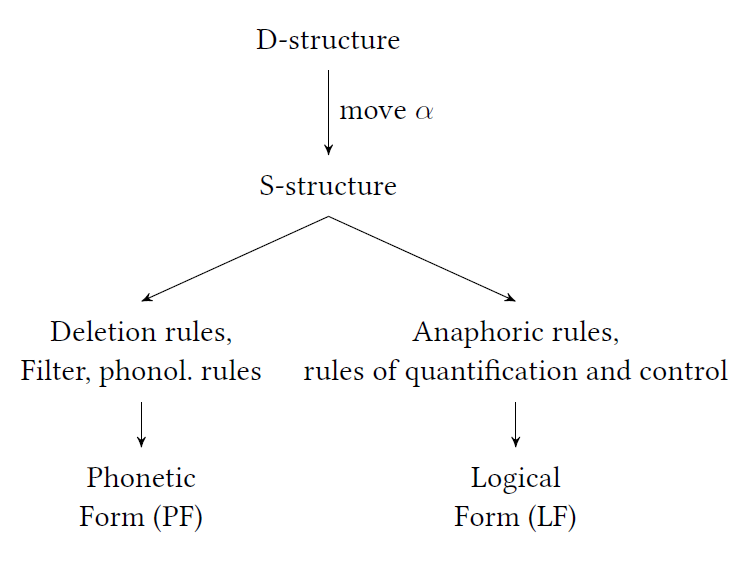
\includegraphics[scale=.45]{material/11tmodell}
	\caption{T-Modell \citep[vgl.][]{MuellerS15b}}
\end{figure}
	
\end{frame}


%%%%%%%%%%%%%%%%%%%%%%%%%%%%%%%%%%
%%%%%%%%%%%%%%%%%%%%%%%%%%%%%%%%%%
\section{Funktionale Phrasen II}
\iftoggle{toc}{
\frame{
\begin{multicols}{2}
\frametitle{~}
	\tableofcontents[currentsection]
\end{multicols}
}
}

%%%%%%%%%%%%%%%%%%%%%%%%%%%%%%%%%%
\begin{frame}
\frametitle{Funktionale Phrasen II}

\begin{itemize}
	\item Bisher \ras Nebensatzstellung im Deutschen
	\item Wann kommt die NS-Stellung vor? \ras Complementizer!
	
	\eal
	\ex[]{(Ich denke,) \alert{dass} Syntax Spaß machen sollte.}
	\ex[]{Syntax \alert{sollte} Spaß machen.}
	\ex[]{(Ich frage mich,) \alert{ob} der Winter jemals enden wird.}
	\ex[]{Der Winter \alert{wird} niemals enden.}
	\ex[*]{Der Winter \alert{ob wird} niemals enden.}
	\zl
	
	\item Complementizer und finite Verben in V2-Sätzen sind komplementär!
	
\end{itemize}

\end{frame}


%%%%%%%%%%%%%%%%%%%%%%%%%%%%%%%%%%
%%%%%%%%%%%%%%%%%%%%%%%%%%%%%%%%%%
\subsection{Complementizer Phrase}
%\frame{
%\frametitle{~}
%	\tableofcontents[currentsection]
%}

%%%%%%%%%%%%%%%%%%%%%%%%%%%%%%%%%%
\begin{frame}
\frametitle{Complementizer Phrase}

\begin{itemize}
	\item Abk.: CP
	\item C nimmt eine IP als Komplement
\end{itemize}

\begin{figure}[b]
%	\begin{minipage}[b]{0.05\textwidth}
%	\hfill
%	\end{minipage} 
	%
	\begin{minipage}[b]{0.45\textwidth}
	\centering
	\tiny{
		\begin{forest}
		sn edges,
		[IP [DP [Peter,triangle]]
			[\MyPxbar{I} [VP 
					[\MyPxbar{V} [DP [den Wagen,triangle]]
						[\zerobar{V} [gekauft]]
						]]
				[I [hat]]
				]
		]
		\end{forest}
		}
		\caption{NS als IP}	
  	\end{minipage}  
  	%  
  	\begin{minipage}[b]{0.05\textwidth}
	\hfill
	\end{minipage}  
	%
	\begin{minipage}[b]{0.45\textwidth}
	\centering
	\tiny{
		\begin{forest}
		sn edges,
[CP	[\MyPxbar{C}	[\zerobar{C} [\alert{dass}\\ \alert{ob}\\ \alert{weil}]]	
		[IP [DP [Peter,triangle]]
			[\MyPxbar{I} [VP
					[\MyPxbar{V} [DP [den Wagen,triangle]]
						[\zerobar{V} [gekauft]]
						]]
				[\zerobar{I} [hat]]
				]
		]
	]
]
		\end{forest}
		}
		\caption{NS als CP}	
  	\end{minipage}  
  	%         
%  	\begin{minipage}[b]{0.05\textwidth}
%	\hfill
%	\end{minipage}  
\end{figure}

\end{frame}


%%%%%%%%%%%%%%%%%%%%%%%%%%%%%%%%%%
\begin{frame}
\frametitle{Complementizer Phrase}

\begin{itemize}
	\item CP ist für den Satzmodus zuständig 
	\begin{itemize}
		\item Eingebetteter Satz
		\item Eingebetteter Fragesatz
		\item Deklarativsatz
		\item E- oder K-Fragesatz
		\item Imperativsatz
	\end{itemize}
\end{itemize}
\end{frame}


%%%%%%%%%%%%%%%%%%%%%%%%%%%%%%%%%%
\begin{frame}
\frametitle{Complementizer Phrase}

\begin{itemize}
	\item CP bestimmt die \textbf{Form} der IP \ras Finit!
\end{itemize}

\begin{figure}[b]
%	\begin{minipage}[b]{0.05\textwidth}
%	\hfill
%	\end{minipage} 
	%
	\begin{minipage}[b]{0.45\textwidth}
	\centering
	\tiny{
		\begin{forest}
		sn edges,
[*CP	[\MyPxbar{C}	[\zerobar{C} [dass]]
		[IP [DP [Peter,triangle]]
			[\MyPxbar{I} [VP 
					[\MyPxbar{V} [DP [den Wagen, triangle]]
						[\zerobar{V} [\alert{kaufen}]]{\draw[<-,red] (.south east)--++(0em,-1.5ex)--++(+2em,0pt)
node[anchor=west,align=center]{infinit};}
						]]
				[\zerobar{I} [$\emptyset$]]
				]
		]
	]
]		
		\end{forest}
		}
		\caption{Ungrammatisch}	
  	\end{minipage}  
  	%  
  	\begin{minipage}[b]{0.05\textwidth}
	\hfill
	\end{minipage}  
	%
	\begin{minipage}[b]{0.45\textwidth}
	\centering
	\tiny{
		\begin{forest}
		sn edges,
[CP	[\MyPxbar{C}	[\zerobar{C} [dass]]	
		[IP [DP [Peter,triangle]]
			[\MyPxbar{I} [VP 
					[\MyPxbar{V} [DP [den Wagen, triangle]]
						[\zerobar{V} [t$_{i}$]]
						]]
				[\zerobar{I} [\alert{kauft}$_{i}$]]{\draw[<-,red] (.south east)--++(0em,-1.5ex)--++(+2em,0pt)
node[anchor=west,align=center]{finit};}
				]
		]
	]
]
		\end{forest}
		}
		\caption{Grammatisch}	
  	\end{minipage}  
  	%         
%  	\begin{minipage}[b]{0.05\textwidth}
%	\hfill
%	\end{minipage}  
\end{figure}

\end{frame}


%%%%%%%%%%%%%%%%%%%%%%%%%%%%%%%%%%
\begin{frame}
\frametitle{Complementizer Phrase}

\begin{itemize}
	\item Korrelation zwischen \textbf{Verbzweit- und Verbletztstruktur}
	\item Kopfbewegung
\end{itemize}


\begin{figure}[b]
%	\begin{minipage}[b]{0.05\textwidth}
%	\hfill
%	\end{minipage} 
	%
	\begin{minipage}[b]{0.45\textwidth}
	\centering
	\tiny{
		\begin{forest}
		sn edges,
[CP	[\MyPxbar{C}	[\zerobar{C} [dass]]{\draw[<-,red] (.south west)--++(0em,-1.5ex)--++(-2em,0pt)
node[anchor=east,align=center]{besetzt! \ras \\ keine I-C-Bewegung};}
		[IP [DP [Peter,triangle]]
			[\MyPxbar{I} [VP 
					[\MyPxbar{V} [DP [den Wagen, triangle]]
						[\zerobar{V} [t$_{i}$]]
						]]
				[\zerobar{I} [kauft$_{i}$]]
				]
		]
	]
]		
		\end{forest}
		}
		\caption{V-I-Bewegung}	
  	\end{minipage}  
  	%  
  	\begin{minipage}[b]{0.05\textwidth}
	\hfill
	\end{minipage}  
	%
	\begin{minipage}[b]{0.45\textwidth}
	\centering
	\tiny{
		\begin{forest}
		sn edges,
[CP	[\MyPxbar{C}	[\zerobar{C} [kauft$_{i}$]]{\draw[<-,red] (.south west)--++(0em,-1.5ex)--++(-2em,0pt)
node[anchor=east,align=center]{frei! \ras \\ I-C-Bewegung};}
		[IP [DP [Peter,triangle]]
			[\MyPxbar{I} [VP 
					[\MyPxbar{V} [DP [den Wagen, triangle]]
						[\zerobar{V} [t$_{i}$]]
						]]
				[\zerobar{I} [t$_{i}$]]
				]
		]
	]
]
		\end{forest}
		}
		\caption{V-I-C-Bewegung}	
  	\end{minipage}  
  	%         
%  	\begin{minipage}[b]{0.05\textwidth}
%	\hfill
%	\end{minipage}  
\end{figure}

\end{frame}


%%%%%%%%%%%%%%%%%%%%%%%%%%%%%%%%%%
\begin{frame}
\frametitle{Complementizer Phrase}

\begin{itemize}
	\item \textbf{Weitere Position} für Verbzweitsätze
	\item Phrasenposition \ras Aber \textbf{nur eine} Phrasenposition
\ea[*]{[Den Wagen] [Peter] kauft gestern.}
\z

\end{itemize}

\begin{figure}[b]
%	\begin{minipage}[b]{0.05\textwidth}
%	\hfill
%	\end{minipage} 
	%
	\begin{minipage}[b]{0.45\textwidth}
	\centering
	\tiny{
		\begin{forest}
		sn edges,
[CP	[DP$_{i}$ [Peter,triangle]]{\draw[<-,red] (.south west)--++(0em,-1.5ex)--++(-2em,0pt)
node[anchor=east,align=center]{Phrase};}
	[\MyPxbar{C}	[\zerobar{C} [kauft$_{ii}$]]
		[IP [t$_{i}$]
			[\MyPxbar{I} [VP 
					[\MyPxbar{V} [DP [den Wagen, triangle]]
						[\zerobar{V} [t$_{ii}$]]
						]]
				[I [t$_{ii}$]]
				]
		]
	]
]		
		\end{forest}
		}
		\caption{Subjektbewegung}	
  	\end{minipage}  
  	%  
  	\begin{minipage}[b]{0.05\textwidth}
	\hfill
	\end{minipage}  
	%
	\begin{minipage}[b]{0.45\textwidth}
	\centering
	\tiny{
		\begin{forest}
		sn edges,
[CP	[DP$_{ii}$ [den Wagen,triangle]]{\draw[<-,red] (.south west)--++(0em,-1.5ex)--++(-2em,0pt)
node[anchor=east,align=center]{Phrase};}
	[\MyPxbar{C}	[\zerobar{C} [kauft$_{i}$]]
		[IP [DP [Peter,triangle]]
			[\MyPxbar{I} [VP 
					[\MyPxbar{V} [t$_{ii}$]
						[\zerobar{V} [t$_{i}$]]
						]]
				[\zerobar{I} [t$_{i}$]]
				]
		]
	]
]
		\end{forest}
		}
		\caption{Objektbewegung}	
  	\end{minipage}  
  	%         
%  	\begin{minipage}[b]{0.05\textwidth}
%	\hfill
%	\end{minipage}  
\end{figure}

\end{frame}


%%%%%%%%%%%%%%%%%%%%%%%%%%%%%%%%%%
\begin{frame}
\frametitle{Complementizer Phrase}

\begin{itemize}
	\item Die CP ist für den \textbf{Satzmodus} und die \textbf{illokutionäre Kraft} zuständig
\end{itemize}

\begin{figure}[b]
%	\begin{minipage}[b]{0.05\textwidth}
%	\end{minipage} 
	%
	\begin{minipage}[b]{0.45\textwidth}
	\centering
	\scriptsize{
		\begin{forest}
		sn edges,
		[CP [$\emptyset$]{\draw[<-,red] (.south west)--++(0em,-1.5ex)--++(-2em,0pt)
node[anchor=east,align=center]{leer};}
			[C' [C [dass]]{\draw[<-,red] (.south west)--++(0em,-1.5ex)--++(-2em,0pt)
node[anchor=east,align=center]{Subjunktion};}
				[IP [Peter den Wagen kauft,triangle]]]]
		\end{forest}
		}
		\caption{Eingebetteter Satz}	
  	\end{minipage}  
  	%  
  	\pause            
	\begin{minipage}[c]{0.07\textwidth}
	\hfill
  	\end{minipage}
  	%         
  	\begin{minipage}[b]{0.40\textwidth}
	\centering
	\scriptsize{
		\begin{forest}
		sn edges,
		[CP [$\emptyset$]{\draw[<-,red] (.south west)--++(0em,-1.5ex)--++(-2em,0pt)
node[anchor=east,align=center]{leer};}
			[C' [C [kauft$_{i}$]]{\draw[<-,red] (.south west)--++(0em,-1.5ex)--++(-2em,0pt)
node[anchor=east,align=center]{Verb};}
				[IP [Peter den Wagen t$_{i}$,triangle]]]]
		\end{forest}
		}
		\caption{Entscheidungsfrage}
  	\end{minipage}  
  	%              
%	\begin{minipage}[b]{0.05\textwidth}
%  	\end{minipage}
  	
\end{figure}

\end{frame}


%%%%%%%%%%%%%%%%%%%%%%%%%%%%%%%%%%
\begin{frame}
\frametitle{Complementizer Phrase}

\begin{itemize}
	\item Die CP ist für den \textbf{Satzmodus} und die \textbf{illokutionäre Kraft} zuständig
\end{itemize}

\begin{figure}[b]
%	\begin{minipage}[b]{0.05\textwidth}
%	\end{minipage} 
	%
	\begin{minipage}[b]{0.45\textwidth}
	\centering
	\scriptsize{
		\begin{forest}
		sn edges,
		[CP [DP$_{ii}$ [was,triangle]]{\draw[<-,red] (.south west)--++(0em,-1.5ex)--++(-2em,0pt)
node[anchor=east,align=center]{W-Wort};}
			[C' [C [kauft$_{i}$]]{\draw[<-,red] (.south west)--++(0em,-1.5ex)--++(-2em,0pt)
node[anchor=east,align=center]{Verb};}
				[IP [Peter t$_{ii}$ t$_{i}$,triangle]]]]
		\end{forest}
		}
		\caption{Konstituentenfrage}	
  	\end{minipage}  
  	%  
  	\pause            
%	\begin{minipage}[c]{0.02\textwidth}
%	\hfill
%  	\end{minipage}
  	%         
  	\begin{minipage}[b]{0.49\textwidth}
	\centering
	\scriptsize{
		\begin{forest}
		sn edges,
		[CP [DP$_{ii}$ [Den Wagen,triangle]]{\draw[<-,red] (.south west)--++(0em,-1.5ex)--++(-2em,0pt)
node[anchor=east,align=center]{Konstituente};}
			[C' [C [kauft$_{i}$]]{\draw[<-,red] (.south west)--++(0em,-1.5ex)--++(-2em,0pt)
node[anchor=east,align=center]{Verb};}
				[IP [Peter t$_{ii}$ t$_{i}$,triangle]]]]
		\end{forest}
		}
		\caption{Aussagesatz}
  	\end{minipage}  
  	%              
%	\begin{minipage}[b]{0.05\textwidth}
%  	\end{minipage}
  	
\end{figure}

\end{frame}


%%%%%%%%%%%%%%%%%%%%%%%%%%%%%%%%%%
%%%%%%%%%%%%%%%%%%%%%%%%%%%%%%%%%%
\section{Erklärungspotential}
\iftoggle{toc}{
\frame{
\begin{multicols}{2}
\frametitle{~}
	\tableofcontents[currentsection]
\end{multicols}
}
}

%%%%%%%%%%%%%%%%%%%%%%%%%%%%%%%%%%%
\begin{frame}
\frametitle{Erklärungspotential}

\begin{itemize}
	\item Warum ist eine \textbf{VP mit Subjekt} nicht möglich?
	\eal 
	\ex[]{\dots\ (dass) [Peter den Wagen \alert{kauft}]$_{IP}$.}
	\ex[*]{\dots\ (dass) [Peter den Wagen \alert{kaufen}]$_{VP}$.}
	\zl

\pause
	\begin{itemize}
		\item \textbf{Kasus} und \textbf{$\theta$-Rolle} werden \textbf{strukturell} vergeben.
		\item[]
		\item Erst durch die \textbf{Subjekt-Verb-Kongruenz} erhält das Subjekt \textsc{nom}-Kasus
		\item[]
		\item Subjekt-Verb-Kongruenz geschieht durch die \textbf{SpecIP-I$^{0}$-Relation} (strukturelle/lokale Relation)
	\end{itemize}
\end{itemize}		

\end{frame}


%%%%%%%%%%%%%%%%%%%%%%%%%%%%%%%%%%%
\begin{frame}
\frametitle{Erklärungspotential}

\begin{itemize}
	\item Warum ist eine \textbf{VP mit Subjekt} nicht möglich?
	\eal 
	\ex[]{\dots\ (dass) [Peter den Wagen \alert{kauft}]$_{IP}$.}
	\ex[*]{\dots\ (dass) [Peter den Wagen \alert{kaufen}]$_{VP}$.}
	\zl

\end{itemize}

\begin{figure}[b]
	\begin{minipage}[b]{0.80\textwidth}
	\centering
	\scriptsize{
		\begin{forest}
		sn edges,
		[IP 
			[DP [Peter,triangle]]{\draw[<-,red] (.north west)--++(0em,+1.5ex)--++(-2em,0pt)
node[anchor=east,align=center]{\textsc{nom}- \& \\ \textsc{akk}-Vergabe};}
			[\MyPxbar{I} 
				[VP 					
					[\MyPxbar{V} 
						[DP [den Wagen, triangle]]{\draw[<-,red] (.north west)--++(0em,+1.5ex)--++(-2em,0pt)
node[anchor=east,align=center]{\textsc{patiens}- \& \\ \textsc{akk}-Vergabe};}
						[\zerobar{V} [gekauft]]
					]
				]
				[\zerobar{I} [hat]]
			]
		]
		\end{forest}
		}
	\caption{Position und Funktion im X-Bar-Schema} 
  	\end{minipage}  
  	%  
%	\begin{minipage}[b]{0.02\textwidth}
%	\hfill
%  	\end{minipage}
  	%   
\end{figure}

\end{frame}


%%%%%%%%%%%%%%%%%%%%%%%%%%%%%%%%%%%
\begin{frame}
\frametitle{Erklärungspotential}


\begin{itemize}
	\item Warum ist die \textbf{Vorfeldbesetzung durch VP mit Subjekt} nicht möglich?
	\eal 
	\ex[]{[Den Wagen \alert{gekauft}]$_{VP}$ hat Peter gestern.}
	\ex[*]{[Peter den Wagen \alert{gekauft}]$_{VP}$ hat gestern.}
	\zl

\pause
	\item Damit das Subjekt sichtbar (overt realisiert) wird, muss es \textbf{in SpecIP} \textsc{nom} \textbf{erhalten} \ras Es ist nicht mehr in der VP!

\end{itemize}		

\pause
\begin{itemize}
	\item \textbf{Gewinn} \ras Elegante und restriktive Theorie \nocite{Haspelmath94a}
	\begin{itemize}
		\item Keine \textbf{Köpfe} ohne Phrasen
		\item Keine \textbf{Phrasen} ohne Köpfe (exozentrische Phrasen)
		\item Strukturelle \textbf{Position} bestimmt Funktion
		\item \textbf{Einheitlichkeit} der X-Bar-Struktur
	\end{itemize}		

\end{itemize}

\end{frame}


%%%%%%%%%%%%%%%%%%%%%%%%%%%%%%%%%%%
\begin{frame}
\frametitle{Erklärungspotential}

\begin{itemize}
	\item \textbf{Grammatikalisierung} \ras ein seltenes Argument \citep{Haspelmath94a}
	\item Hilfsverben, Tempus- und Aspektaffixe werden \textbf{aus Vollverben} grammatikalisiert \ras \textbf{Unterschied zwischen Wort oder Affix} ist nicht von Bedeutung
	\item[]
	\item Die \textbf{Kopf-Dependent-Relation} bleibt bei der Grammatikalisierung immer erhalten \ras Hilfsverben und weitere Affixe sind Köpfe 
\end{itemize}


\begin{figure}[b]
%	\begin{minipage}[b]{0.05\textwidth}
%	\end{minipage} 
	%
	\begin{minipage}[b]{0.40\textwidth}
	\centering
	\footnotesize{
		\begin{forest}
		sn edges,
		[VP [DP [Julia,triangle]]
			[\MyPxbar{V} [VP [cantare,triangle]]
				[\zerobar{V} [\alert{habet}]]		{\draw[<-,red] (.south east)--++(0em,-1.5ex)--++(+2em,0pt)
node[anchor=west,align=center]{Kopf};}
			]
		]
		\end{forest}
		}
		\caption{Latein}	
  	\end{minipage}  
  	%  
  	\pause            
	\begin{minipage}[c]{0.07\textwidth}
	\hfill
  	\end{minipage}
  	%         
  	\begin{minipage}[b]{0.40\textwidth}
	\centering
	\footnotesize{
		\begin{forest}
		sn edges,
		[IP [DP [Julia,triangle]]
			[\MyPxbar{I} [VP [cant-,triangle]]
				[\zerobar{I} [\alert{-ará}]]{\draw[<-,red] (.south east)--++(0em,-1.5ex)--++(+2em,0pt)
node[anchor=west,align=center]{Kopf};}
			]
		]
		\end{forest}
		}
		\caption{Spanisch}
  	\end{minipage}  
  	%              
%	\begin{minipage}[b]{0.05\textwidth}
%  	\end{minipage}
  	
\end{figure}


\end{frame}


%%%%%%%%%%%%%%%%%%%%%%%%%%%%%%%%%%
%%%%%%%%%%%%%%%%%%%%%%%%%%%%%%%%%%
\section{Mehr funktionale Kategorien}
\only<presentation>{
\iftoggle{toc}{
\frame{
\begin{multicols}{2}
\frametitle{~}
	\tableofcontents[currentsection]
\end{multicols}
}
}
}

%%%%%%%%%%%%%%%%%%%%%%%%%%%%%%%%%%%
\begin{frame}
\only<presentation>{\frametitle{Mehr funktionale Kategorien}}
\nocite{Lenerz93a}

\begin{figure}[b]
	\begin{minipage}[b]{0.48\textwidth}
	\begin{figure}					
		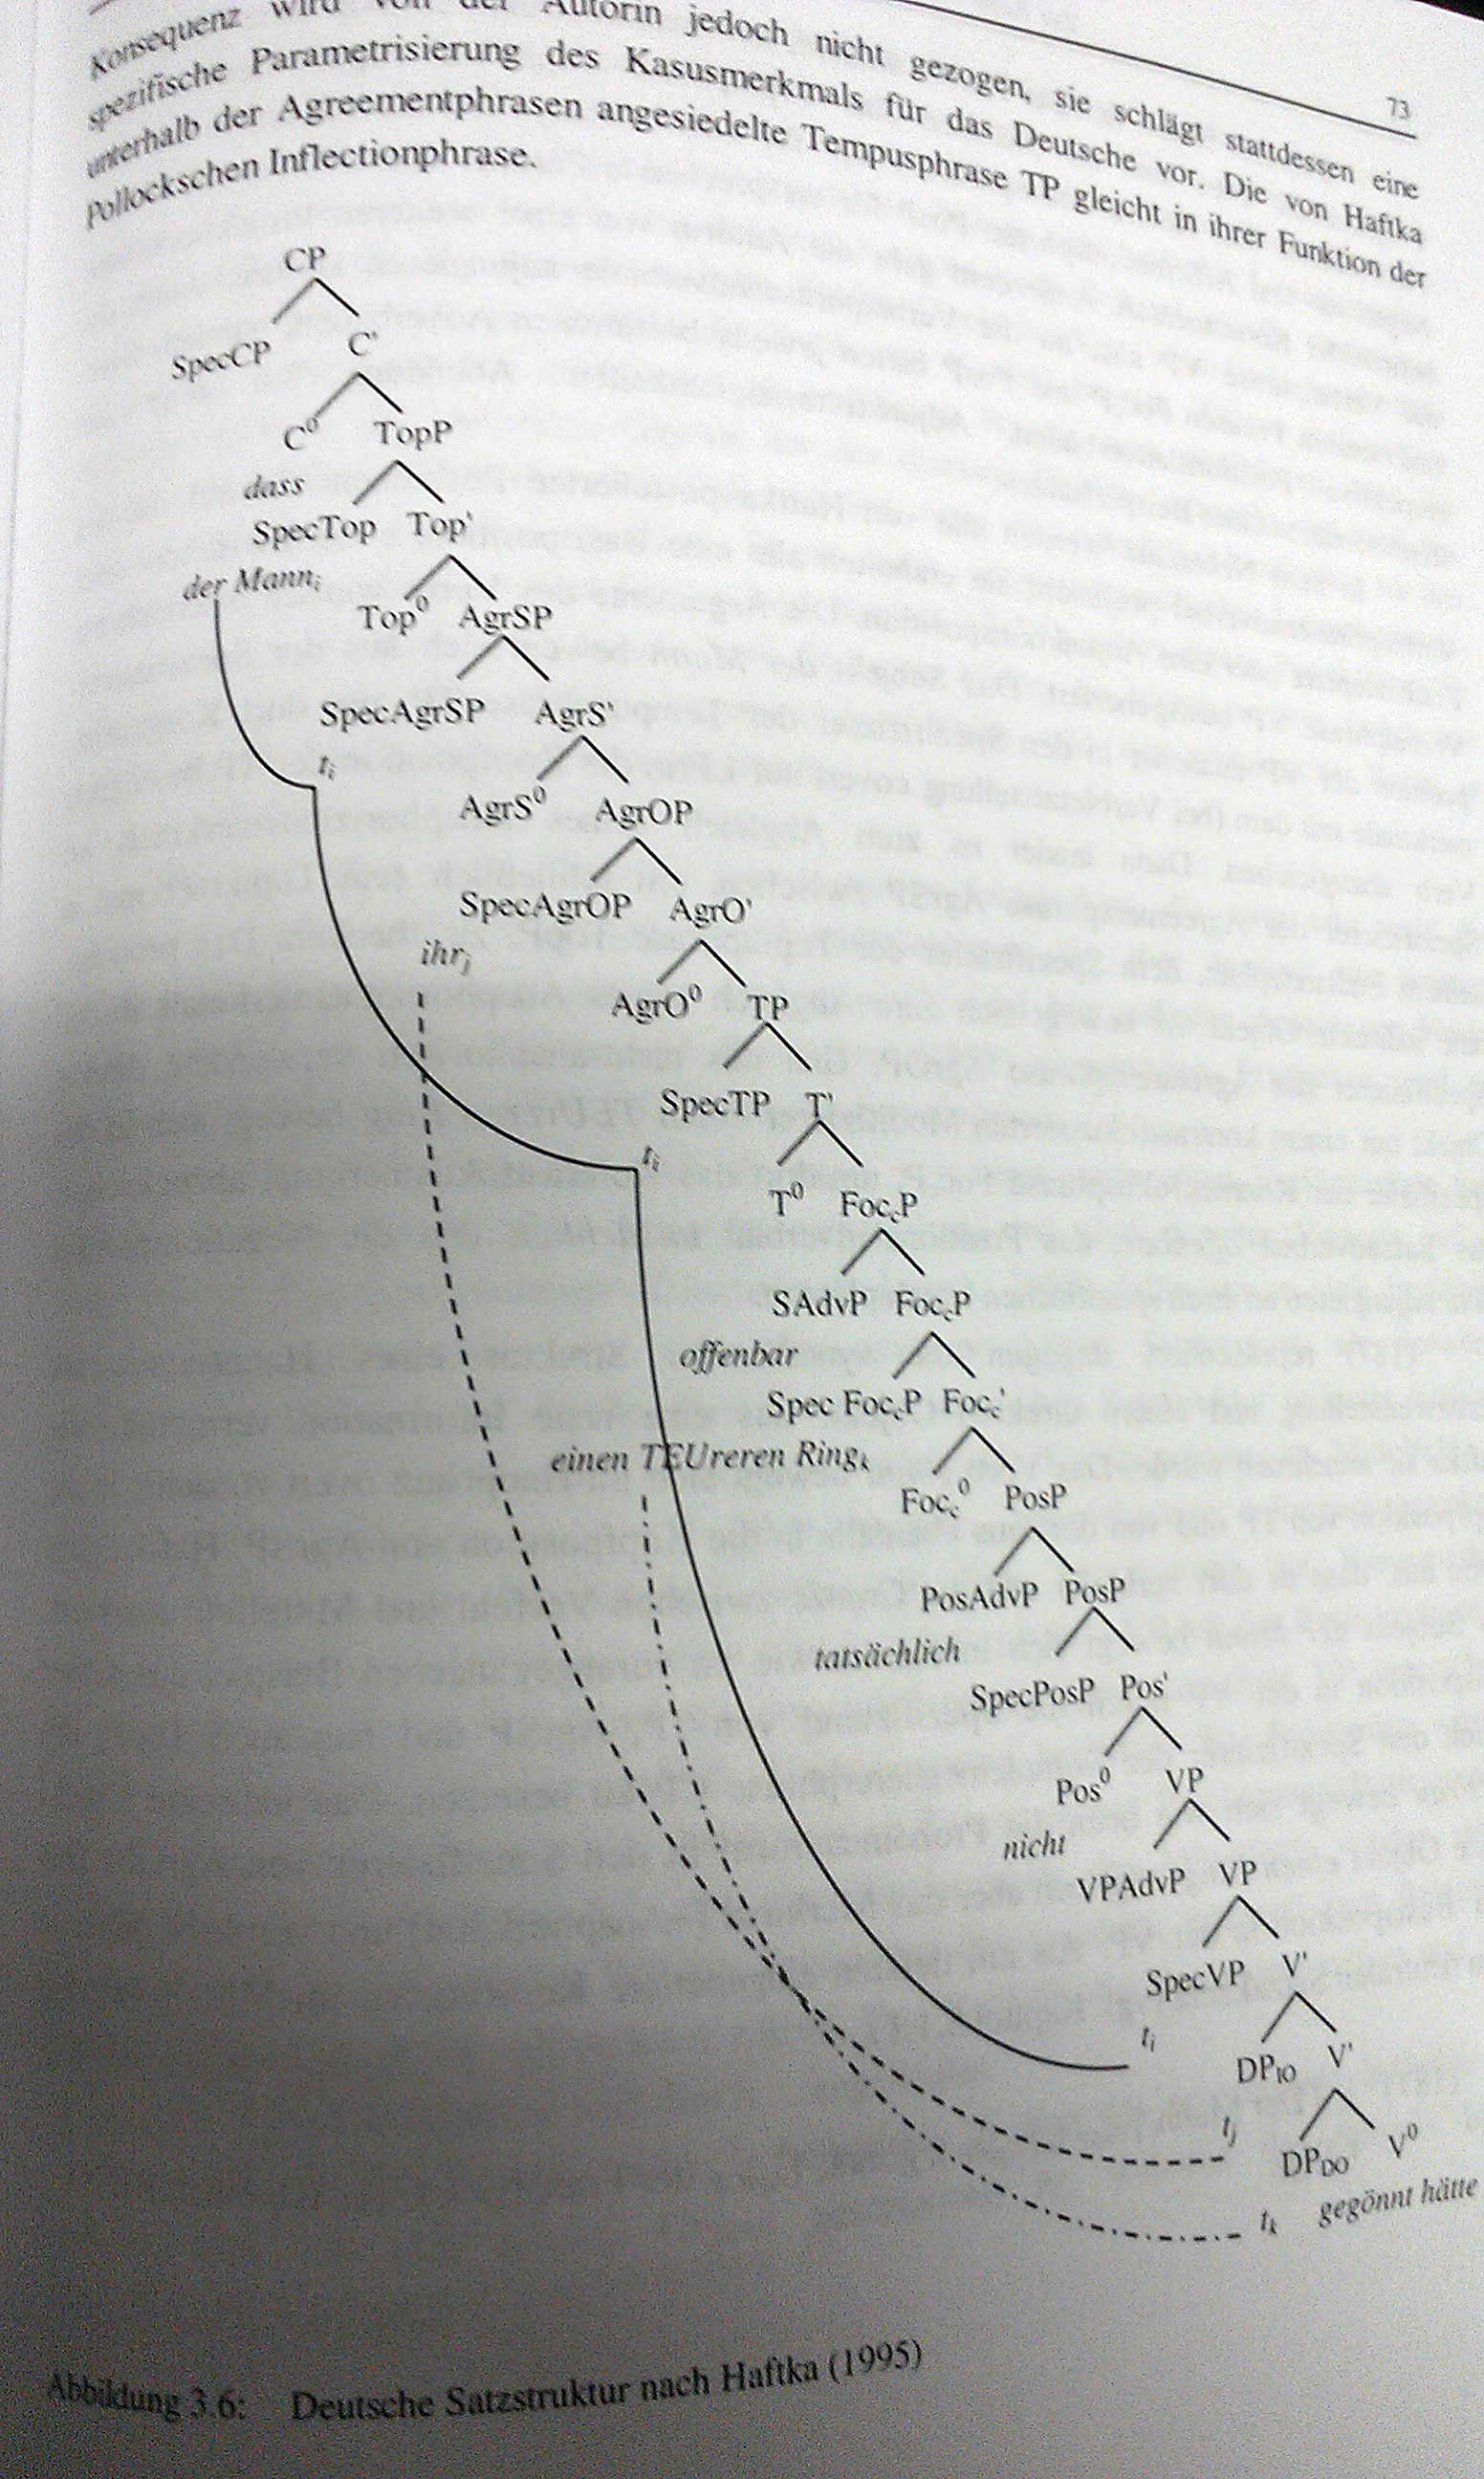
\includegraphics[scale=0.07]{material/Haftka95CP}
		\caption{Struktur der CP (Haftka 95)}
		%\label{Zeichen1}
	\end{figure}
	\end{minipage}
	%
%	\begin{minipage}[b]{0.20\textwidth}
  	%	
%	\end{minipage}
	%				
	\begin{minipage}[b]{0.48\textwidth}
	\begin{figure}
		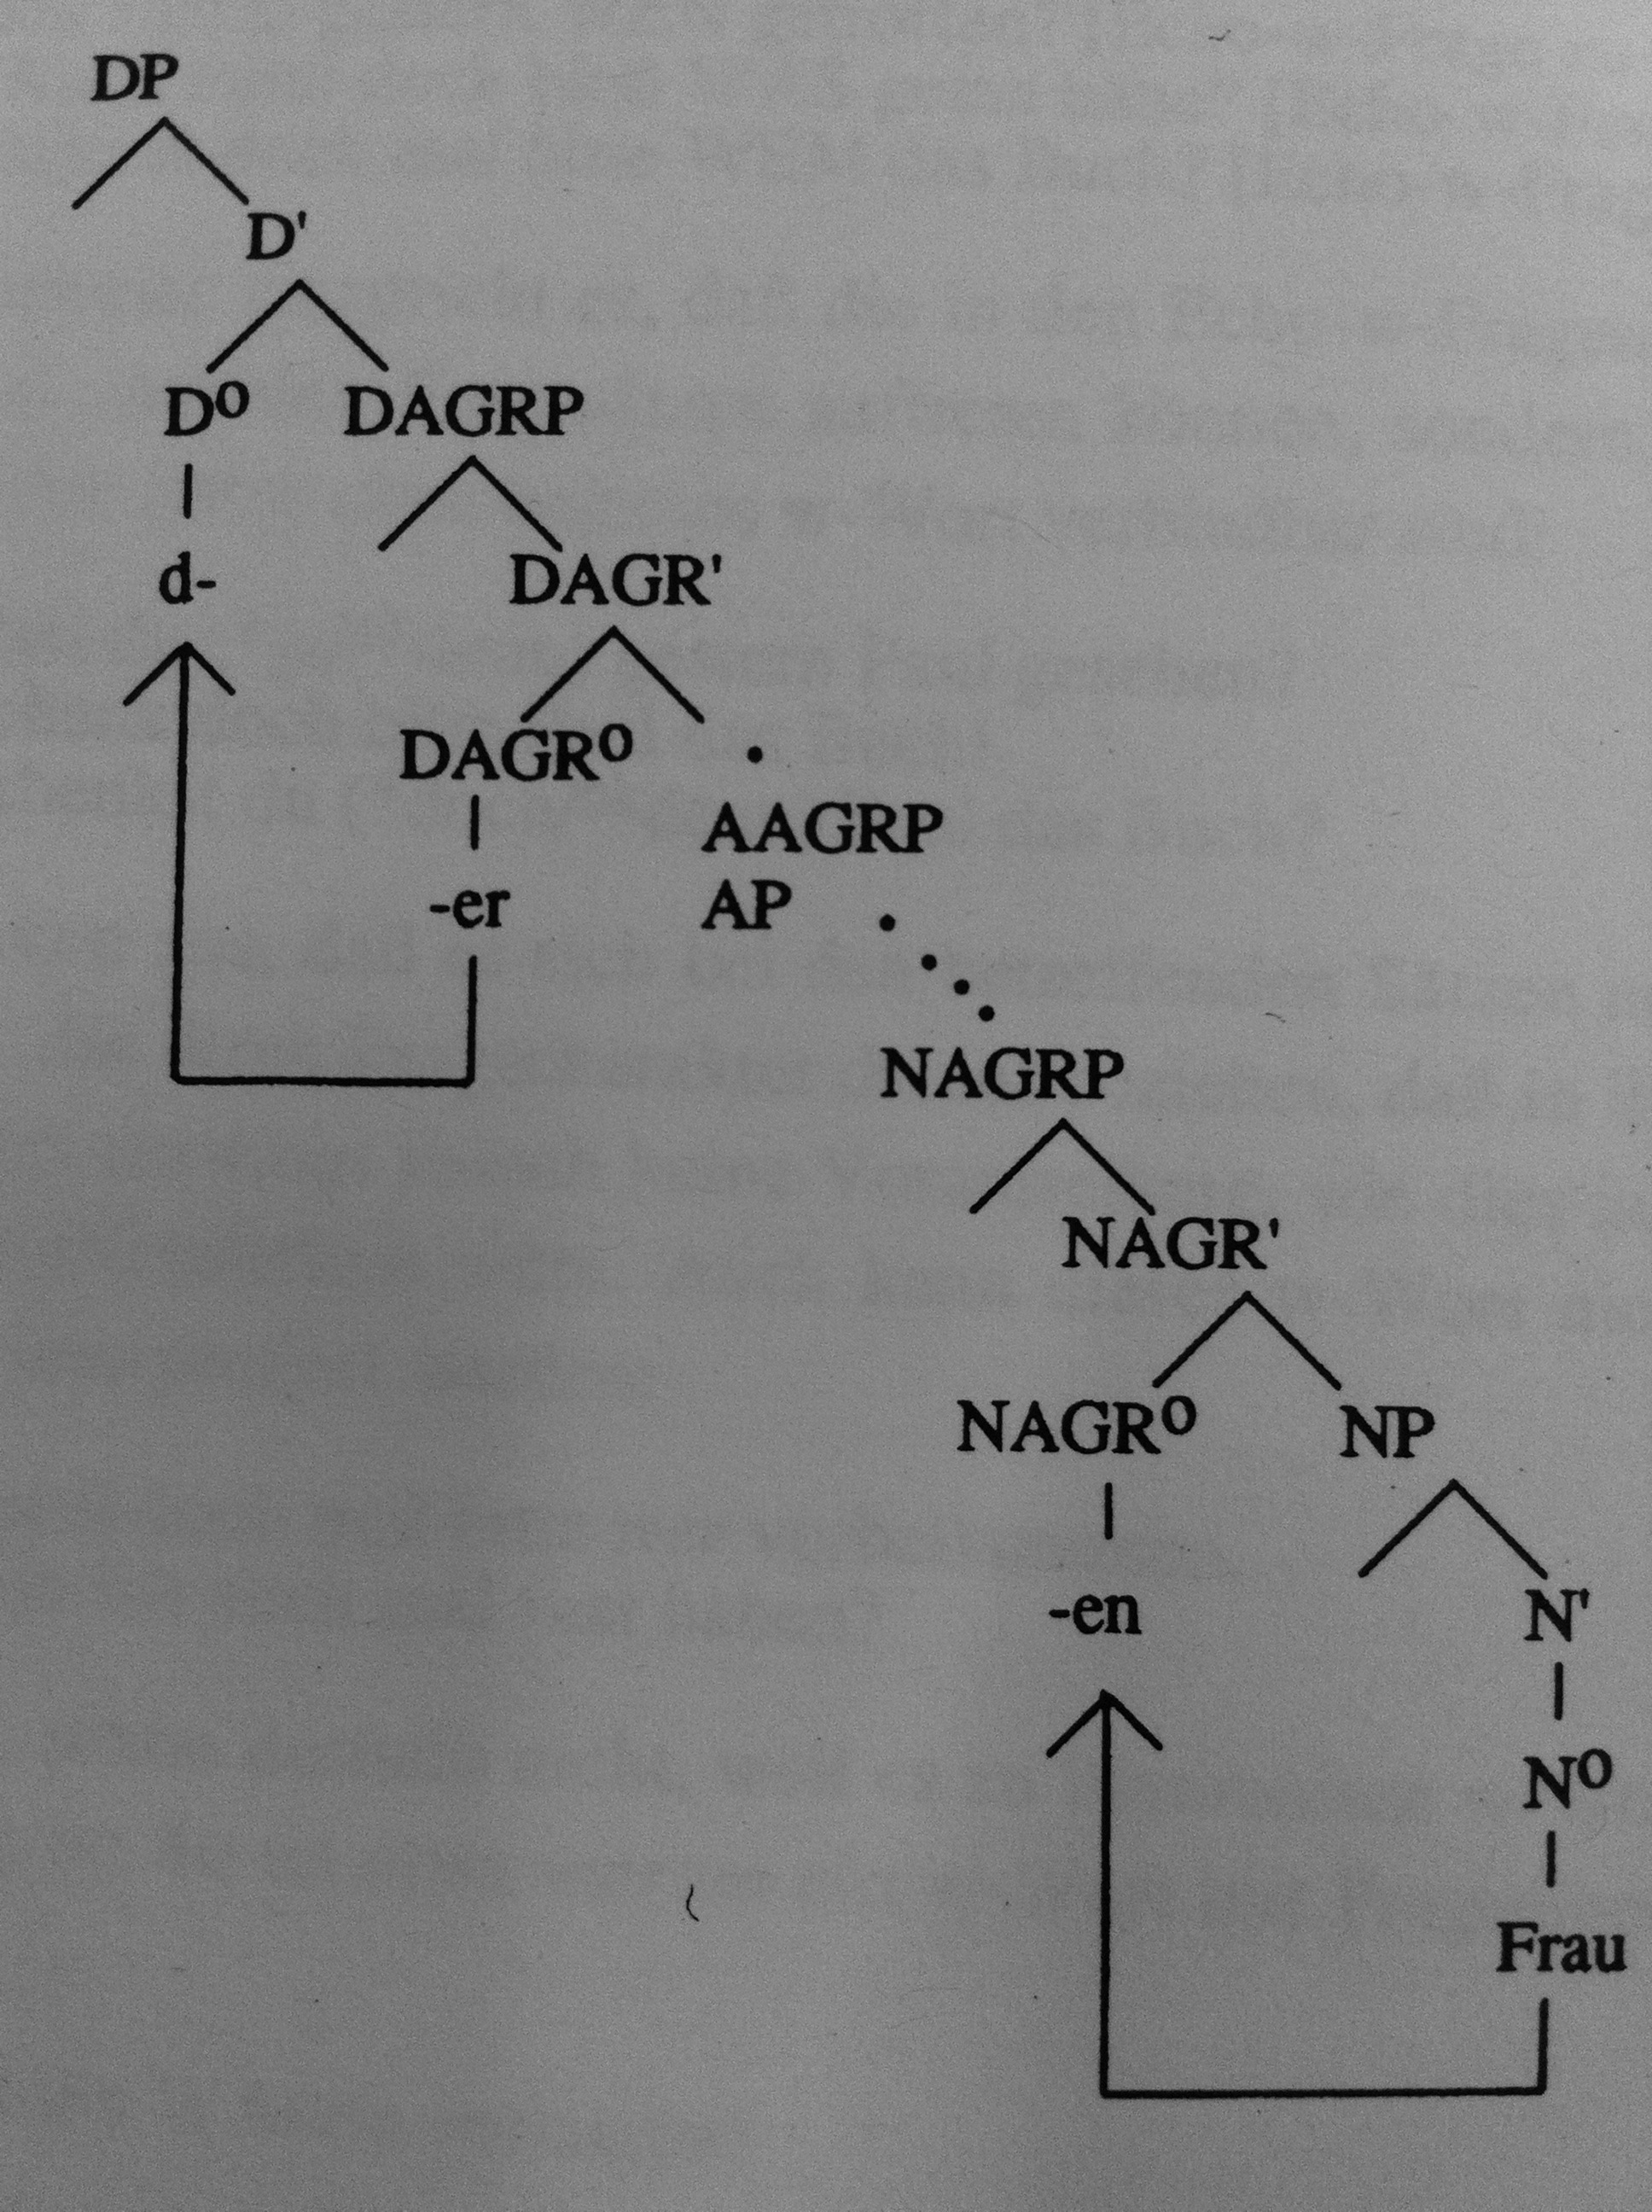
\includegraphics[scale=0.07]{material/Lenerz93DP}
		\caption{Struktur der DP (Lenerz 93)}
		%\label{Zeichen2}
	\end{figure}
	\end{minipage}                        
\end{figure}

\end{frame}


%%%%%%%%%%%%%%%%%%%%%%%%%%%%%%%%%%
%%%%%%%%%%%%%%%%%%%%%%%%%%%%%%%%%%
\section{Übungen}
\iftoggle{toc}{
\frame{
\begin{multicols}{2}
\frametitle{~}
	\tableofcontents[currentsection]
\end{multicols}
}
}

\iftoggle{uebung}{
%%%%%%%%%%%%%%%%%%%%%%%%%%%%%%%%%%
\begin{frame}
\frametitle{Übungen}

\begin{itemize}
	\item Analysieren Sie die folgenden Phrasen nach dem X-Bar-Schema.


\eal
\ex Peter schläft.
\ex Wer schläft?
\ex Gebe ich dir ein großes Stück Kuchen?
\ex die kurz vor dem Mittagessen aufgestellte Speisekarte
\zl
 

\item Erklären Sie mithilfe des X-Bar-Schemas die Ambiguität im folgenden Satz:

\ea Das Kind küsst die Mama.
\z

\item Erklären Sie mithilfe des X-Bar-Schemas, warum der folgende Satz ungrammatisch ist:

\ea Im Auto ich habe heute geschlafen.
\z


\end{itemize}
\end{frame}

}
%%%%%%%%%%%%%%%%%%%%%%%%%%%%%%%%%%
\iftoggle{loesung}{

\begin{frame}
\frametitle{Lösungen}
\begin{figure}[b]
	%
	\begin{minipage}[b]{0.45\textwidth}
	\centering
	\scalebox{0.6}{
		\begin{forest}
		sn edges,
		[CP 
			[DP$_{k}$ [Peter,triangle]
			]
			[\MyPxbar{C}
				[\zerobar{C} [schläft$_{i}$]
				]
				[TP [t$_{k}$]
					[\MyPxbar{T}
						[VP [\MyPxbar{V} [\zerobar{V} [t$_{i}$	]]]]
						[\zerobar{T} [t$_{i}$]]
					]
				]
			]
		]
		\end{forest}
		}
  	\end{minipage}  
  	%            
  	%         
  	\begin{minipage}[b]{0.45\textwidth}
	\centering
	\scalebox{0.6}{
		\begin{forest}
		sn edges,
		[CP 
			[DP$_{k}$ [Wer,triangle]
			]
			[\MyPxbar{C}
				[\zerobar{C} [schläft$_{i}$]
				]
				[TP [t$_{k}$]
					[\MyPxbar{T}
						[VP [\MyPxbar{V} [\zerobar{V} [t$_{i}$	]]]]
						[\zerobar{T} [t$_{i}$]]
					]
				]
			]
		]
		\end{forest}
		}
  	\end{minipage}  
  	%              
%	\begin{minipage}[b]{0.05\textwidth}
%  	\end{minipage}
  	
\end{figure}

\end{frame}


%%%%%%%%%%%%%%%%%%%%%%%%%%%%%%%%%%
\begin{frame}
\frametitle{Lösungen}
\begin{figure}[b]
	%
	\begin{minipage}[b]{0.45\textwidth}
	\centering
	\scalebox{0.6}{
		\begin{forest}
		sn edges,
		[CP 
			[\MyPxbar{C}
				[\zerobar{C} [Gebe$_{i}$]
				]
				[TP [ich]
					[\MyPxbar{T}
						[VP [\MyPxbar{V} 
								[DP [dir,triangle]]								
								[\xxbar{V}
										[DP [ein großes Stück Kuchen,triangle]]		
										[\zerobar{V} [t$_{i}$]]]]]
						[\zerobar{T} [t$_{i}$]]
					]
				]
			]
		]
		\end{forest}
		}
  	\end{minipage}  
  	%            
  	%         
  	\begin{minipage}[b]{0.45\textwidth}
	\centering
	\scalebox{0.6}{
		\begin{forest}
		sn edges,
		[DP
			[\MyPxbar{D}
				[\zerobar{D}[die]]
				[NP
					[AP
						[PP 
							[kurz vor dem Mittagessen, triangle]
%							[AdvP [\MyPxbar{Adv} [\zerobar{Adv} [kurz]]]]
%							[PP [\MyPxbar{P}
%									[\zerobar{Adv} [vor]]
%									[DP [\MyPxbar{D} [\zerobar{D} [dem]]
%										[NP [\MyPxbar{N} [\zerobar{N} [Mittagessen]]]]
%										]
%									]				
%								]							
%							]
						]	
						[AP [\MyPxbar{A} [\zerobar{A} [aufgestellte]]]]
					]
					[NP [\MyPxbar{N} [\zerobar{N} [Speisekarte]]]
					]
				]
			]
		]
		\end{forest}
		}
  	\end{minipage}  
  	%              
%	\begin{minipage}[b]{0.05\textwidth}
%  	\end{minipage}
  	
\end{figure}

\end{frame}


%%%%%%%%%%%%%%%%%%%%%%%%%%%%%%%%%%

\begin{frame}
\frametitle{Lösungen}

\begin{figure}[b]
%
\begin{minipage}[b]{0.45\textwidth}
\centering
\scalebox{0.6}{
\begin{forest}
sn edges,
[CP
	[DP$ _{k} $[Das Kind, triangle]]
	[\MyPxbar{C} 
		[\zerobar{C}[küsst$ _{i} $]]
		[TP
			[t$ _{k} $]
			[\MyPxbar{T}
				[VP [\MyPxbar{V}
						[DP[die Mama, triangle]]
						[\zerobar{V}[t$ _{i} $]]
					]
				]
				[\zerobar{T}[t$ _{i} $]]
			]
		]
	]
]
\end{forest}
(Das Kind ist Subjekt.)}
\end{minipage}
%
\begin{minipage}[b]{0.45\textwidth}
\centering
\scalebox{0.6}{
\begin{forest}
sn edges,
[CP
	[DP$ _{k} $[Das Kind, triangle]]
	[\MyPxbar{C} 
		[\zerobar{C}[küsst$ _{i} $]]
		[TP
			[DP[die Mama, triangle]]
			[\MyPxbar{T}
				[VP [\MyPxbar{V}
						[t$ _{k} $]
						[\zerobar{V}[t$ _{i} $]]
					]
				]
				[\zerobar{T}[t$ _{i} $]]
			]
		]
	]
]
\end{forest}
(Das Kind ist Objekt.)}
\end{minipage}
%
\end{figure}
\end{frame}

%%%%%%%%%%%%%%%%%%%%%%%%%%%%%%%%%%
\begin{frame}
\frametitle{Lösungen}
\begin{figure}[b]
	%
	\begin{minipage}[b]{0.45\textwidth}
	\centering
	\scalebox{0.6}{
		\begin{forest}
		sn edges,
		[CP
			[DP$_{k}$ [Ich,triangle]]
			[\MyPxbar{C} [\zerobar{C} [habe$_{i}$]]
				[TP [t$_{k}$]
					[\MyPxbar{T}
						[VP	[AdVP [heute,triangle]]
							[VP [PP	[im Auto,triangle]]{\draw[->,red] (.north west)--++(-7em,0em)--++(0em,14em)
node[anchor=east,align=center]{SpecCP schon besetzt, \\PP kann sich nicht dahin bewegen};}
								[\MyPxbar{V} [\zerobar{V} [geschlafen t$_{i}$]]]
							]
						]
						[\zerobar{T} [t$_{i}$]]
					]
				]
			]	
		]
		\end{forest}
		}
  	\end{minipage}  
  	%            
  	%         
  	\begin{minipage}[b]{0.45\textwidth}
	\hfill
  	\end{minipage}  
  	%              
%	\begin{minipage}[b]{0.05\textwidth}
%  	\end{minipage}
  	
\end{figure}

\end{frame}

}
%%%%%%%%%%%%%%%%%%%%%%%%%%%%%%%%%%
\iftoggle{uebung}{

\begin{frame}
\frametitle{Übungen}

\begin{itemize}
\item Geben Sie an, welches Wort sich in der Kopfposition der folgenden Phrasen befindet:

\eal
\ex viele besorgte Mütter
\ex den Menschen in Not helfen
\ex Wasser ohne Kohlensäure
\ex auf Maria warten
\ex ob sie heute kommen werden
\ex Sophie ihren Traummann gefunden hat
\zl

\end{itemize}

\end{frame}

}
%%%%%%%%%%%%%%%%%%%%%%%%%%%%%%%%%%
\iftoggle{loesung}{

\begin{frame}
\frametitle{Lösungen}

\eal
\ex viele besorgte \textbf{Mütter} (NP)
\ex den Menschen in Not \textbf{helfen} (VP)
\ex \textbf{Wasser} ohne Kohlensäure (NP)
\ex auf Maria \textbf{warten} (VP)
\ex \textbf{ob} sie heute kommen werden (CP)
\ex Sophie ihren Traummann gefunden \textbf{hat} (TP)
\zl

\end{frame}

}
%%%%%%%%%%%%%%%%%%%%%%%%%%%%%%%%%%%%%%%%%%%%%%%%%%%%%%%%%%%%%%%%%%%%%%%%%%%%%%%%%%
\iftoggle{uebung}{

\begin{frame}
\only<presentation>{\frametitle{Übungen}}

\begin{itemize}
	\item Was ist an dieser Struktur misslungen? Beziehen Sie sich in Ihrer Antwort auf die in der Sitzung behandelten Köpfigkeitsmerkmale und Strukturaufbaugesetzmäßigkeiten.
\end{itemize}

\begin{figure}
	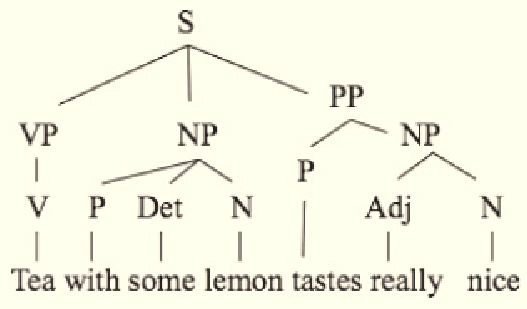
\includegraphics[scale=.5]{material/wrongtree}
	\caption{\url{http://specgram.com/CLXV.1/05.cruz-ferreira.know22.html}}
\end{figure}
	
\end{frame}

}
%%%%%%%%%%%%%%%%%%%%%%%%%%%%%%%%%%%%%%%%%%%%%%%%%%%%%%%%%%%
\iftoggle{loesung}{

\begin{frame}
\frametitle{Lösung}

\begin{itemize}
\item keine binäre Struktur (mehr als zwei Töchter)
\item Konstituenten falsch bestimmt (\zB Tea = V?) 
\item Köpfe nicht erkennbar
\end{itemize}

}
%%%%%%%%%%%%%%%%%%%%%%%%%%%%%%%%%%
\begin{frame}

\begin{figure}
	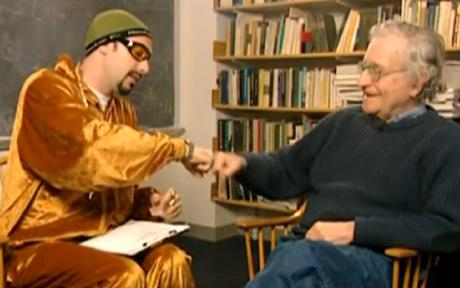
\includegraphics[scale=.5]{material/11chomksy}
	\caption{Geschafft!}
\end{figure}
	
\end{frame}

